\documentclass[10pt]{article}

%Math
\usepackage{amsmath}
\usepackage{amsfonts}
\usepackage{amssymb}
\usepackage{amsthm}
\usepackage{ulem}
\usepackage{stmaryrd} %f\UTF{00FC}r Blitz!

\usepackage{wrapfig}

%PageStyle
\usepackage[ngerman]{babel} % deutsche Silbentrennung
\usepackage[utf8]{inputenc} 
\usepackage{fancyhdr, graphicx}
\usepackage[scaled=0.92]{helvet}
\usepackage{enumitem}
\usepackage{parskip}
\usepackage[a4paper,top=2cm]{geometry}
\setlength{\textwidth}{17cm}
\setlength{\oddsidemargin}{-0.5cm}


% Shortcommands
\newcommand{\Bold}[1]{\textbf{#1}} %Boldface
\newcommand{\Kursiv}[1]{\textit{#1}} %Italic
\newcommand{\T}[1]{\text{#1}} %Textmode
\newcommand{\Nicht}[1]{\T{\sout{$ #1 $}}} %Streicht Shit durch
\usepackage{tabto} %Möglichkeit Tabulatoren zu nutzen%

%Arrows
\newcommand{\lra}{\leftrightarrow} 
\newcommand{\ra}{\rightarrow}
\newcommand{\la}{\leftarrow}
\newcommand{\lral}{\longleftrightarrow}
\newcommand{\ral}{\longrightarrow}
\newcommand{\lal}{\longleftarrow}
\newcommand{\Lra}{\Leftrightarrow}
\newcommand{\Ra}{\Rightarrow}
\newcommand{\La}{\Leftarrow}
\newcommand{\Lral}{\Longleftrightarrow}
\newcommand{\Ral}{\Longrightarrow}
\newcommand{\Lal}{\Longleftarrow}

% Code listenings
\usepackage{color}
\usepackage{xcolor}
\usepackage{listings}
\usepackage{caption}
\DeclareCaptionFont{white}{\color{white}}
\DeclareCaptionFormat{listing}{\colorbox{gray}{\parbox{\textwidth}{#1#2#3}}}
\captionsetup[lstlisting]{format=listing,labelfont=white,textfont=white}
\lstdefinestyle{JavaStyle}{
 language=Java,
 basicstyle=\footnotesize\ttfamily, % Standardschrift
 numbers=left,               % Ort der Zeilennummern
 numberstyle=\tiny,          % Stil der Zeilennummern
 stepnumber=5,              % Abstand zwischen den Zeilennummern
 numbersep=5pt,              % Abstand der Nummern zum Text
 tabsize=2,                  % Groesse von Tabs
 extendedchars=true,         %
 breaklines=true,            % Zeilen werden Umgebrochen
 frame=b,         
 %commentstyle=\itshape\color{LightLime}, Was isch das? O_o
 %keywordstyle=\bfseries\color{DarkPurple}, und das O_o
 basicstyle=\footnotesize\ttfamily,
 stringstyle=\color[RGB]{42,0,255}\ttfamily, % Farbe der String
 keywordstyle=\color[RGB]{127,0,85}\ttfamily, % Farbe der Keywords
 commentstyle=\color[RGB]{63,127,95}\ttfamily, % Farbe des Kommentars
 showspaces=false,           % Leerzeichen anzeigen ?
 showtabs=false,             % Tabs anzeigen ?
 xleftmargin=17pt,
 framexleftmargin=17pt,
 framexrightmargin=5pt,
 framexbottommargin=4pt,
 showstringspaces=false      % Leerzeichen in Strings anzeigen ?        
}

%Config
\renewcommand{\headrulewidth}{0pt}
\setlength{\headheight}{15.2pt}

%Metadata
\fancyfoot[C]{If you use this documentation for a exam, you should offer a beer to the authors!}
\title{
	\vspace{5cm}
	Verteilte Systeme - Zusammenfassung
}
\author{Florian Thiévent}
\date{4. Semester (FS 2019)}


% hier beginnt das Dokument
\begin{document}

% Titelbild
\maketitle
\thispagestyle{fancy}

\newpage

% Inhaltsverzeichnis
\pagenumbering{Roman}
\tableofcontents	  	


\newpage
\setcounter{page}{1}
\pagenumbering{arabic}

% Inhalt Start

\section{Networking}
\subsection{InetAddress}
\subsubsection*{Static factory methods}
\begin{itemize}
	\item getByName(String name)
	\item getByAddress (4/16 bytes)
	\item getAllByName(String host)
	\item getLocalHost()
\end{itemize}
\subsubsection*{Instance methods}
\begin{itemize}
	\item byte[] getAddress()
	\item String getHostAddress()
	\item String getHostName()
	\item String getCanonicalHostName()
	\item boolean isReachable(int timeout)
	\item boolean isMulticastAddress()
\end{itemize}
\subsection{Network Interfaces}
\begin{lstlisting}[language=Java, caption=Network Interfaces and its addresses, style=JavaStyle]
public static void main(String[] args) throws SocketException {
	Enumeration<NetworkInterface> interfaces = NetworkInterface.getNetworkInterfaces();
	while(interfaces.hasMoreElements()){
		NetworkInterface intf = interfaces.nextElement();
		Syst	em.out.print(intf.getName());
		System.out.println(" ["+intf.getDisplayName()+"]");
		Enumeration<InetAddress> adr = intf.getInetAddresses();
		while(adr.hasMoreElements()){
			System.out.println("\t" + adr.nextElement());
		}
		byte[] hardwareAddress = intf.getHardwareAddress();
	}
}
\end{lstlisting}
\subsection{Sockets}
Abstraction through which an application may send and receive data through the network. A Socket is identified by Hostname/IP and port number.
\begin{description}
	\item[Stream Sockets] \hfill
	\begin{itemize}
		\item Use TCP as end-to-end protocol
		\item Provide a reliable byte-stream
		\item Connection oriented: Socket represents one end of a TCP connection
	\end{itemize}
	\item[Datagaram Sockets] \hfill 
	\begin{itemize}
		\item Use UDP as protocol
		\item Not connection oriented, not reliable
	\end{itemize}
\end{description}
\subsubsection{Controlling Socket Behaviors}
\begin{description}
	\item[Blocking \& Timeouts] \hfill 
	\begin{description}
		\item[ServerSocket.accept / InputStream.read] \hfill \\
			read or accept call will not block for more than a fixed number of msec otherwise, InterruptedIOException is thrown (get/setSoTimeout(int timeout))
		\item[Socket constructor] \hfill \\
			Uses a system-defined timeout, cannot be changed by Java API (Solution: use connect)
		\item[OutputStream.write] \hfill \\
			Cannot be interrupted / caused to time-out by Java API
	\end{description}
	\item[Keep-Alive] \hfill
	\begin{itemize}
		\item TCP provides a keep-alive mechanism
		\item Probe messages are sent after a certain time
		\item Application only sees keep-alive working if the probes fail!
		\item Per default keep-alive is disabled
		\item Default timeout: 2h (7200 secs)
	\end{itemize}
	\item[Send / Receive Buffer Size] \hfill
	\begin{itemize}
		\item When a Socket is created, the OS must allocate buffers to hold incoming \& outgoing data
		\item Receive buffer size may also be specified on server socket (for accepted
sockets which immediately receive data)
	\end{itemize}
	\item[No Delay] \hfill
	\begin{itemize}
		\item TCP tries to avoid sending small packets
		\item Buffers data until it has more to send, combines small packets with larger ones
		\item Necessary if application has to be efficient
		\item Default: false
	\end{itemize}
\end{description}
\subsubsection{Closing Connections}
\begin{description}
	\item[close()] \hfill 
	\begin{itemize}
		\item Once an endpoint (client or server) closes the socket, it can no longer send or receive data	
		\item Close can only be used to signal the other end that the caller is completely finished communicating
	\end{itemize}
	\item[shutdownOutput()] \hfill
	\begin{itemize}
		\item Closes output-stream, no more data can be may be written (IOException)
		\item All data written before shutdownOutput can be read by receiver
	\end{itemize}
	\item[shutdownInput()] \hfill
	\begin{itemize}
		\item Closes the input stream
		\item Any undelivered data is (silently) discarded, read operations will return -1
	\end{itemize}
	\item[s.close() / s.shutdownOutput()] \hfill
	\begin{itemize}
		\item Data may still be waiting to be delivered to the other side
		\item By default, socket tries to deliver remaining data, but if socket crashes, data may be lost without notification to sender (as close returns immediately)
	\end{itemize}
\end{description}
\subsubsection{User Datagram Protocol}
\begin{itemize}
	\item UDP allows to address applications over ports
	\item UDP adds another layer of addressing (ports) to that of IP
	\item UDP detects some form of data corruption that may occur in transit and discards corrupted messages
	\item UDP retains message boundaries
\end{itemize}

\newpage
\section{Internet}
\subsection{Protocol}
\begin{description}	
	\item[GET] \hfill
	\begin{itemize}
		\item Access of content from the server
		\item Idempotent, i.e. the side effects of N>0 identical requests is the same as for a single request ( f(f(x)) = f(x) )
	\end{itemize}
	\item[POST] \hfill \\
		Comparable to GET but Method must not necessarily be idempotent and Request data is transferred in the body of the request
	\item[HEAD] \hfill
	\begin{itemize}
		\item Identical to GET, except that the server must not return the body
		\item Can be used to request meta information (headers) about the resource
	\end{itemize}
	\item[OPTIONS (1.1)] \hfill \\
		Returns information about the communication options available on the specified resource (or on the server in general if request URI=*)
	\item[PUT (1.1)] \hfill \\
		Stores a web page on the server (rarely implemented)
	\item[DELETE (1.1)] \hfill \\
		Removes a web resource from the servver (rarely implemented)
	\item[TRACE (1.1)] \hfill \\
		Returns the request as it was accepted by server ($\Ra$ debugging)
	\item[CONNECT (1.1)] \hfill \\
		Implemented by Proxy Server capable to provide an SSL tunnel
\end{description}
\subsubsection{Response Codes}
\begin{description}
	\item[200-299: Success] \hfill
	\begin{itemize}
		\item[200] OK
		\item[201] Created
		\item[202] Accepted
	\end{itemize}
	\item[300-399: Redirections] \hfill
	\begin{itemize}
		\item[300] Multiple Choices
		\item[301] Moved Permanently
		\item[302] Found
		\item[303] See Other (e.g. after POST)
		\item[304] Not Modified
		\item[305] Use Proxy
		\item[307] Temporary Redirect
	\end{itemize}
	\item[400-499: Client Error] \hfill
	\begin{itemize}
		\item[400] Bad Request
		\item[401] Unauthorized
		\item[402] Payment Required
		\item[403] Forbidden
		\item[404] Not Found
		\item[405] Method Not Allowed
		\item[407] Proxy Authentication Required
		\item[408] Request Time-out
		\item[411] Length Required
		\item[413] Request Entity Too Large
		\item[414] Request-URI Too Large
		\item[415] Unsupported Media Type
	\end{itemize}
	\item[500-599: Server Error] \hfill
	\begin{itemize}
		\item[500] Internal Server Error
		\item[501] Not Implemented
		\item[503] Service Unavailable
		\item[505] HTTP Version not supported
	\end{itemize}
\end{description}
\subsection{Request Headers}
\begin{description}
	\item[Host] server host 
	\item[Referer] host from which the request is initiated
	\item[Accept] data types supported by the client 
	\item[Accept-Language] language supported by client
	\item[Accept-Encoding] encodings supported by client, e.g. gzip or deflate
	\item[User-Agent] browser details, supplies server with information about the type of browser making the request
	\item[Connection: Keep-Alive] browser is requesting the use of persistent TCP connections
\end{description}
\subsection{Response Headers}
\begin{description}
	\item[Content-Type] MIME-Type of content
	\item[Content-Length] size of body (in bytes)
	\item[Content-Encoding] compression algorithms
	\item[Location] used by redirections
	\item[Date] timestamp when the response was created 
	\item[Last-Modified] modification date of resource (assumed by server) 
	\item[Expires] date after which the result is considered stale 
	\item[Server] information about the server
	\item[Transfer-Encoding] specifies type of transformation
	\item[Cache-Control] information about cache handling (e.g. no-cache disables caching)
	\item[WWW-Authenticate] information about authentication method
\end{description}
\subsection{Servlet}
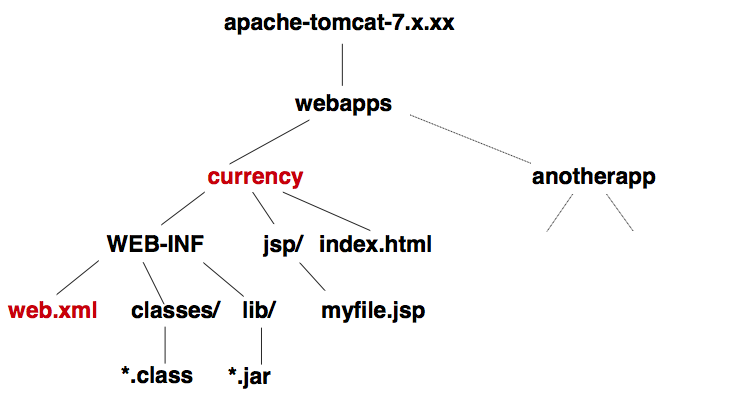
\includegraphics[scale=0.5]{images/tomcat-structure.png}
\begin{lstlisting}[language=Java, caption=Servlet Example, style=JavaStyle]
public class Converter extends HttpServlet {
	public void doGet(HttpServletRequest request, HttpServletResponse response) throws IOException {
		response.setContentType("text/html");
		PrintWriter out = response.getWriter();
		String amount = request.getParameter("amt"); 
		String from = request.getParameter("from"); 
		String to = request.getParameter("to"); 
		String res = computeResult(amount, from, to);
		out.println("<html>\n<body bgcolor=\"white\">"); 
		out.println("<h1>Currency Converter</h1>"); 
		out.println(amount + " " + from + " = " + res);
		out.println("</body>\n</html>");
	}
	String computeResult(String amount, String from, String to){...}
}
\end{lstlisting}
\begin{lstlisting}[language=Java, caption=web.xml, style=JavaStyle]
<?xml version="1.0" encoding="ISO-8859-1"?>
<web-app xmlns="http://java.sun.com/xml/ns/javaee" xmlns:xsi="http://www.w3.org/2001/XMLSchema-instance" xsi:schemaLocation="http://java.sun.com/xml/ns/javaee http://java.sun.com/xml/ns/javaee/web-app_3_0.xsd" version="3.0">
    <servlet>
        <servlet-name>CurrencyConverter</servlet-name>
        <servlet-class>ch.fhnw.ds.Converter</servlet-class>
    </servlet>
    <servlet-mapping>
        <servlet-name>CurrencyConverter</servlet-name>
		<url-pattern>/convert</url-pattern>
	</servlet-mapping>
</web-app>
\end{lstlisting}

\newpage
\section{Webservices}
\subsection{XML-RPC}

simples RPC Protokoll über HTTP, benötigt keine lange Einarbeitungszeit
\subsubsection{Primitive Datentypen}
\begin{itemize}
\item int, i4 \tab signed 32bit Integer
\item string \tab ASCII string (no latin1)
\item boolean \tab either 0 or 1
\item double \tab double-precision floating point number
\item dateTime.iso8601 \tab z.B. 20050717T14:08:14
\item base64 \tab raw binary data, base64 encoded
\end{itemize}

\begin{lstlisting}[language=Java, caption=Beispiele, style=JavaStyle]
<i4>13</i4>
<boolean>0</boolean>
\end{lstlisting}

\subsubsection{Structs}
\begin{itemize}
\item Struct enthält Members mit Name und Wert.
\item können rekursiv sein (Structs die Structs enthalten)
\end{itemize}

\begin{lstlisting}[language=Java, caption=Struct Beispiel, style=JavaStyle]
<i4>13</i4>
<struct> 
  <member> 
    <name>from</name> 
    <value><i4>-5</i4></value> 
  </member> 
  <member> 
    <name>to</name> 
    <value><i4>5</i4></value> 
  </member>
</struct>
\end{lstlisting}

\subsubsection{Arrays}
\begin{itemize}
\item Element-Typen können gemischt werden
\end{itemize}

\begin{lstlisting}[language=Java, caption=Array, style=JavaStyle]
<array>
 <data>
  <value><i4>-5</i4></value>
  <value><string>44</string></value>
  <value><boolean>1</boolean></value>
 </data> 
</array>
\end{lstlisting}

\subsubsection{XML-RPC Request}
\begin{lstlisting}[language=Java, caption=Method Call, style=JavaStyle]
<?xml version="1.0" encoding="UTF-8"?>
<methodCall>
  <methodName>Echo.getEcho</methodName>
    <params>
      <param>
        <value>World</value>
      </param>
    </params>
</methodCall>
\end{lstlisting}

\subsubsection{XML-RPC Response}
\begin{lstlisting}[language=Java, caption=Single Result, style=JavaStyle]
<?xml version="1.0" encoding="UTF-8"?>
<methodResponse>
  <params>
    <param>
      <value>Hello World, welcome to XML-RPC</value>
    </param>
  </params>
</methodResponse>
\end{lstlisting}
Als Resultat kann nur ein Wert zurückkommen, dieser kann jedoch auch ein Struct oder ein Array sein.

\begin{lstlisting}[language=Java, caption=Fault Result, style=JavaStyle]
<?xml version="1.0" encoding="UTF-8"?>
<methodResponse>
  <fault>
    <value>
      <struct>
        <member>
          <name>faultCode</name>
          <value><i4>0</i4></value>
        </member>
        <member>
          <name>faultString</name>
          <value>No such handler: Echo.foo</value>
        </member>
      </struct>
    </value>
  </fault>
</methodResponse>
\end{lstlisting}

\subsubsection{Apache XML-RPC Sample Server}
\lstinputlisting[language=java,caption=Sample Server,style=JavaStyle]{code/ApacheXML-RPC-Server1.class}

\lstinputlisting[language=java,caption=Handler Class Server,style=JavaStyle]{code/ApacheXML-RPC-Server2.class}

Nur Instanzmethoden der Handlerklasse sind zugreifbar. Keine void Methoden. Public Default Constructor zwingend.

\subsubsection{Apache XML-RPC Client}
\lstinputlisting[language=java,caption=Handler Class Server,style=JavaStyle]{code/ApacheXML-RPC-Client.class}


\subsection{SOAP}
\subsubsection{WSDL (Web Services Description Language)}
(früher Web Services Definition Language)\linebreak
WSDL ist eine XML basierte Interface Beschreibungssprache die genutzt wird um die Funktionalität von Webservices zu beschreiben. Eine WSDL Beschreibung eines Webservices enthält:
\begin{itemize}
\item Wie der Service aufgerufen werden kann
\item Welche Parameter er erwartet
\item Welche Datenstruktur er zurückgibt
\end{itemize}

\subsubsection{JAX-WS (Java API for XML Web Services}
JAX-WS ist eine Java API um Webservices zu erstellen. Es ist Teil der Java EE (Enterprise Edition) Plattform von Sun Microsystems. Wie auch andere Java EE APIs nutzt JAX-WS Annotationen (@Webservice, @WebMethod usw). Basiert auf SOAP. Nur WSDL 1.1 unterstützt.

\subsubsection{Anleitung JAX-WS}
1. Interface erstellen
\begin{lstlisting}[language=Java, caption=Interface erstellen, style=JavaStyle]
package ch.fhnw.ds.jaxws.server;
import javax.jws.WebService;
@WebService
public interface HelloService {
	String sayHello(@WebParam(name = "name") String name);
}
\end{lstlisting}

2. Interface implementieren
\begin{lstlisting}[language=Java, caption=Interface implementieren, style=JavaStyle]
package ch.fhnw.ds.jaxws.server; 
import java.util.Date; 
@WebService 
public class HelloServiceImpl implements HelloService { 
	@Override 
	public String sayHello(@WebParam(name = "name") String name){ 
		return "Hello " + name + " from SOAP at " + new Date(); 
	} 
}
\end{lstlisting}
3. Java Objekte für XML Requests \& Responses generieren
\% wsgen -cp bin -keep -s src -d bin ch.fhnw.ds.jaxws.server.HelloServiceImpl
\begin{itemize}
\item cp <path> classpath
\item keep keep generated files
\item s <path> path where to place generated source files
\item d <path> path where to place generated output files
\item <SEI> specify a SIB (service implementation bean)
\end{itemize}
\begin{lstlisting}[language=Java, caption=SayHello, style=JavaStyle]
package ch.fhnw.ds.jaxws.server.jaxws;
import ...;
@XmlRootElement(name = "sayHello", 
		namespace = "http://server.jaxws.ds.fhnw.ch/")
@XmlAccessorType(XmlAccessType.FIELD)
@XmlType(name = "sayHello",
		namespace = "http://server.jaxws.ds.fhnw.ch/")
public class SayHello {

	@XmlElement(name = "name", namespace = "")
	private String name;
	public String getName() { return this.name; }
	public void setName(String name) { this.name = name; }
}

\end{lstlisting}
\begin{lstlisting}[language=Java, caption=SayHelloResponse, style=JavaStyle]
package ch.fhnw.ds.jaxws.server.jaxws;
import ...;
@XmlRootElement(name = "sayHelloResponse",
		namespace = "http://server.jaxws.ds.fhnw.ch/")
@XmlAccessorType(XmlAccessType.FIELD)
@XmlType(name = "sayHelloResponse",
		namespace = "http://server.jaxws.ds.fhnw.ch/")
public class SayHelloResponse {

	@XmlElement(name = "return", namespace = "")
	private String _return;
	public String getReturn() { return this._return; }
	public void setReturn(String _return) {
		this._return = _return;
	}
}
\end{lstlisting}
4. Service publishen
\begin{lstlisting}[language=Java, caption=HelloServicePublisher, style=JavaStyle]
package ch.fhnw.ds.jaxws.server;
import javax.xml.ws.Endpoint;

public class HelloServicePublisher {
	public static void main(String[] args){
		Endpoint.publish(
			"http://127.0.0.1:9876/hs", // publication URI
			new HelloServiceImpl()); // SIB instance
		System.out.println("service published");
	}
}
\end{lstlisting}

5. Generierte Webservice Definition anschauen
http://localhost:9876/hs?wsdl
\begin{lstlisting}[language=Java, caption=WSDL, style=JavaStyle]
<?xml version="1.0" encoding="UTF-8"?> <definitions 	xmlns:soap="http://schemas.xmlsoap.org/wsdl/soap/" 	xmlns:tns="http://server.jaxws.ds.fhnw.ch/" 	xmlns:xsd="http://www.w3.org/2001/XMLSchema" 	xmlns="http://schemas.xmlsoap.org/wsdl/" 	targetNamespace="http://server.jaxws.ds.fhnw.ch/" 	name="HelloServiceImplService"> 
<types> 
	<xsd:schema> 
		<xsd:import namespace="http://server.jaxws.ds.fhnw.ch/" schemaLocation="http://localhost:9876/hs?xsd=1"> 
		</xsd:import> 
	</xsd:schema> 
</types>
<message name="sayHello">
<part name="parameters"
element="tns:sayHello">
</part>
</message>
<message name="sayHelloResponse">
<part name="parameters"
element="tns:sayHelloResponse">
</part>
</message>
<portType name="HelloServiceImpl">
<operation name="sayHello">
<input message="tns:sayHello"></input>
<output message="tns:sayHelloResponse"></output>
</operation>
</portType>
<binding name="HelloServiceImplPortBinding" 
type="tns:HelloServiceImpl"> 
<soap:binding 
transport="http://schemas.xmlsoap.org/soap/http" 
style="document"> 
</soap:binding> 
<operation name="sayHello"> 
<soap:operation soapAction=""></soap:operation> 
<input> 
<soap:body use="literal"></soap:body> 
</input> 
<output> 
<soap:body use="literal"></soap:body> 
</output> 
</operation> 
</binding>
<service name="HelloServiceImplService">
<port name="HelloServiceImplPort"
binding="tns:HelloServiceImplPortBinding">
<soap:address location="http://localhost:9876/hs">
</soap:address>
</port>
</service>
</definitions>

Referenzierte Schema Definition:

<?xml version="1.0" encoding="UTF-8"?>
<xs:schema xmlns:tns="http://server.jaxws.ds.fhnw.ch/" xmlns:xs="http://www.w3.org/2001/XMLSchema"
version="1.0"
targetNamespace="http://server.jaxws.ds.fhnw.ch/">
<xs:element name="sayHello" type="tns:sayHello"></xs:element> <xs:element name="sayHelloResponse" type="tns:sayHelloResponse"></xs:element> 
<xs:complexType name="sayHello">
  <xs:sequence> 
    <xs:element name="name" type="xs:string" minOccurs="0"></xs:element> 
  </xs:sequence> 
</xs:complexType> 
<xs:complexType name="sayHelloResponse"> 
  <xs:sequence> 
    <xs:element name="return" type="xs:string" minOccurs="0"></xs:element> 
  </xs:sequence>
 </xs:complexType> 
</xs:schema>

\end{lstlisting}

6. Client Proxy generieren
\% wsimport -keep -p ch.fhnw.ds.jaxws.client.jaxws -d bin -s src 
\begin{itemize}
\item -keep keep generated files
\item -p <package> specify (overwrite) target package
\item -s <path> path where to place generated source files
\item -d <path> path where to place generated output files
\item <WSDL> Web Service Definition
\item => HelloServiceImpl generated interface
\item => HelloServiceImplService factory class
\end{itemize}


7. Client Applikation schreiben
\begin{lstlisting}[language=Java, caption=Client, style=JavaStyle]
package ch.fhnw.imvs.client;
import ch.fhnw.imvs.client.jaxws.HelloServiceImpl;
import ch.fhnw.imvs.client.jaxws.HelloServiceImplService;

public class Client {
	public static void main(String[] args) {
		HelloServiceImplService service =
			new HelloServiceImplService();
		HelloServiceImpl port =
			service.getHelloServiceImplPort();
		String result = port.sayHello("Dominik");
		System.out.println(result);
	}
}
\end{lstlisting}

8. JAX-WS HTTP Request
\begin{lstlisting}[language=Java, caption=..., style=JavaStyle]
POST /hs HTTP/1.1						HTTP Request
Accept: text/xml, multipart/related
User-Agent: JAX-WS RI 2.2.4-b01
Host: 127.0.0.1:9877
Connection: keep-alive
Content-Length: 209
Content-Type: text/xml; charset=utf-8		SOAP HTTP Binding
SOAPAction: "http://server.jaxws.ds.fhnw.ch/HelloServiceImpl/sayHelloRequest"

<?xml version="1.0" ?>					SOAP Payload
<S:Envelope xmlns:S="http://schemas.xmlsoap.org/soap/envelope/">
	<S:Body>
		<ns2:sayHello xmlns:ns2="http://server.jaxws.ds.fhnw.ch/">
			<name>Dominik</name>
		</ns2:sayHello>
	</S:Body>
</S:Envelope>


\end{lstlisting}
9. JAX-WS HTTP Response
\begin{lstlisting}[language=Java, caption=..., style=JavaStyle]
HTTP/1.1 200 OK						HTTP Response
Transfer-encoding: chunked
Content-type: text/xml; charset=utf-8
Date: Mon, 18 Mar 2013 00:06:44 GMT
Content-Length: 277

<?xml version="1.0" ?>					SOAP Payload
<S:Envelope xmlns:S="http://schemas.xmlsoap.org/soap/envelope/">
<S:Body>
<ns2:sayHelloResponse
xmlns:ns2="http://server.jaxws.ds.fhnw.ch/">
<return>
Hello Dominik from SOAP at Mon Mar 18 01:06:44 CET 2013
</return>
</ns2:sayHelloResponse>
</S:Body>
</S:Envelope>

\end{lstlisting}

\subsection{Vergleich SOAP und XML-RPC}
\begin{tabular}{|c|c|c|}
\hline 
Feature & XML-RPC & SOAP \\ 
\hline
Structs & yes & yes \\ 
\hline 
Arrays & yes & yes \\ 
\hline 
Named structs \& arrays & no & yes \\ 
\hline 
Short learning curve & yes & no \\ 
\hline 
Developer specified character set & no & yes \\ 
\hline 
Developer defined data types & no & yes \\ 
\hline 
Can specify recipient & no & yes \\ 
\hline 
Require client understanding & no & yes \\ 
\hline 
Message specific processing instructions & no & yes \\ 
\hline  
\end{tabular} 

\newpage
\section{Representation State Transfer (REST)}
\subsection{Prinzipien}
\begin{itemize}
	\item Addressability - Give everything an ID
	\item Uniform, Constrained Interface
	\item Representation-oriented
	\item Link things together - Use Resource references
	\item Stateless communications - Resources hold state
	\item Use standard HTTP methods
\end{itemize}
\subsubsection{Addressability}
\begin{itemize}
	\item Resources = key abstractions in REST
	\item Each resource is addressable via a URI
\end{itemize}
\begin{lstlisting}[language=Java, caption=REST example, style=JavaStyle]
http://www.example.com/customers/1234 http://www.example.com/customers?lastName=Meier http://www.example.com/orders/2011/03/445245 http://www.example.com/products/ http://www.example.com/products/4711
\end{lstlisting}
\subsubsection{CRUD}
\begin{description}
	\item[READ] \hfill
	\begin{itemize}
		\item HTML: \textbf{GET, HEAD}
		\item Retrieve information in a particular representation
		\item No side effects, possibly cached
		\item May contain query parameters
	\end{itemize}
	\item[CREATE] \hfill
	\begin{itemize}
		\item HTML: \textbf{POST}
		\item Create a new sub-resource (without known ID)
	\end{itemize}
	\item[CREATE \& UPDATE] \hfill
	\begin{itemize}
		\item HTML: \textbf{PUT}
		\item Update an existing resource
		\item Create a new resource with a known ID
	\end{itemize}
	\item[DELETE] \hfill
	\begin{itemize}
		\item HTML: \textbf{DELETE}
		\item Remove resources
	\end{itemize}
	\item[OPTIONS] \hfill \\
	Returns allowed operations
\end{description}
\subsubsection{Representation-oriented}
Allow multiple representations of a resource: 
\begin{itemize}
	\item text/html
	\item text/plain
	\item application/json
	\item application/xml
\end{itemize}
\subsubsection{Link things together}
References to other resources may be used in representations
\begin{lstlisting}[language=Java, caption=example, style=JavaStyle]
<order>
   <date>16.03.2013</date>
   <amount>23</amount>
   <product ref="http://example.com/products/4711" />
   <customer ref="http://example.com/customers/1234" />
</order>
\end{lstlisting}

\subsection{SOAP vs REST}
\begin{tabular}{l | l}
	\textbf{REST} & \textbf{SOAP} \\
	\hline
	Resource Oriented & Service oriented \\
	Messages represented in different formats & Messages represented in XML \\
	HTTP used as protocol & Can be bound to different protocols \\
	HTTP verbs are used for access and manipulation & Access and Manipulation is service specific \\
	HTTP error codes are used as error messages & Fault Elements in SOAP body describes errors \\
	No formal interface description language & WSDL is used as interface description language \\
	GET requests can be cached in a proxy & All requests are POST requests, no caching!
\end{tabular}
\begin{center}
	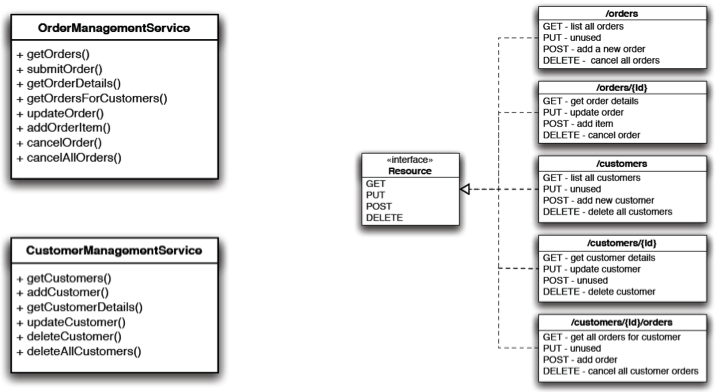
\includegraphics[scale=0.5]{images/soap-rest.png}
\end{center}

\subsection{JAX-RS}
\subsubsection{HTTP Methods}
\begin{itemize}
	\item Annotate resource class methods with HTTP method annotations @GET, @POST, @PUT, @DELETE, @HEAD
	\item Java method name has no significance
	\item Return value is mapped to the response (void = no response)
\end{itemize}

\begin{lstlisting}[language=Java, caption=JAX-RS Service = Annotated Java Class, style=JavaStyle]
@Singleton
@Path("/polls")
public class DoodlePoolResource {
	@GET
	@Path("{id}")
	public String getPoll(@PathParam("id") String key){ ... }
	
	@PUT
	@Path("{id}")
	public String putPoll(@PathParam("id") String key){ ... }
	
	@DELETE
	@Path("{id}")
	public void deletePoll(@PathParam("id") String key){ ... }
}
\end{lstlisting}
\subsubsection{Injection}
\begin{itemize}
	\item Automatic Type Conversion from Strings to
	\begin{itemize}
		\item Primitive types (int, short, float, double, byte, char, boolean)
		\item Classes T which have a constructor with a single String parameter
		\item Classes T which contain a static method T valueOf(String arg)
	\end{itemize}
	\item Default values may be defined with @DefaultValue for the case that the parameter is not passed with the request
\end{itemize}
\begin{description}
	\item[PathParam] \hfill \\
		Allows to extract values from URI template parameters
	\item[MatrixParam] \hfill \\
		Allows to extract matrix parameters ( /images/cars;color=blue/2010/)
	\item[QueryParam] \hfill \\
		Allows to extract query parameters added to a URI
	\item[FormParam] \hfill \\
		Allows to extract values from posted form data
	\item[HeaderParam] \hfill \\
		Allows to extract request headers
	\item[CookieParam] \hfill \\
		Allows to extract values from HTTP cookies
\end{description}
\subsubsection{Content Negotiation}
\begin{description}
	\item[@Produces] declares type of result, default: all types are supported \\
		@Produces(\{"{}text/plain", "{}text/html"\})
	\item[@Consumes] declares type which is accepted (PUT / POST) \\
		@Consumes("{}application/x-www-form-urlencoded")
\end{description}
\subsection{Data Binding}
\begin{lstlisting}[language=Java, caption=XStream Provider, style=JavaStyle]
@Provider
@Consumes("application/xstream")
@Produces("application/xstream")
public class XStreamProvider implements MessageBodyReader<Object>, MessageBodyWriter<Object>{
	private XStream xstream = new XStream(new DomDriver());
	
	public boolean isReadable(Class<?> type, Type genericType, Annotation[] annotations, MediaType mimeType) {
		return true;
	}
	public Object readFrom(Class<Object> type, Type genericType, Annotation[] annotations, MediaType mimeType, MultivaluedMap<String, String> httpHeaders, InputStream entityStream) {
		return xstream.fromXML(entityStream);
	}
	public boolean isWriteable(Class<?> type, Type genericType, Annotation[] ann, MediaType mimeType) {
		return true;
	}
	
	public long getSize(Object object, Class<?> type, Type genericType, Annotation[] ann, MediaType mimeType) {
		return -1;// size not yet known
	}
	
	public void writeTo(Object object, Class<?> type, Type genericType, Annotation[] ann, MediaType mimeType, MultivaluedMap<String, Object> httpHeaders, OutputStream entityStream) {
		xstream.toXML(object, entityStream);
	}
}
\end{lstlisting}
\begin{lstlisting}[language=Java, caption=XStream Example, style=JavaStyle]
public class Client {
	public static void main(String[] args) {
	ClientConfig config = new DefaultClientConfig();
	config.getClasses().add(XStreamProvider.class);
	Client c = Client.create(config);
	WebResource r = c.resource("http://localhost:9998/msg");
	Msg msg = new Msg("Hello from XClient");
	r.type("application/xstream").put(msg);
	Msg res = r.accept("application/xstream").get(Msg.class); 
	System.out.println(res);
	System.out.println(res.getText());
	System.out.println(res.getDate());
	}
}
\end{lstlisting}
\subsection{JAXB}
Java Architecture for XML Binding, kurz JAXB, ist eine Programmschnittstelle in Java, die es ermöglicht, Daten aus einer XML-Schema-Instanz heraus automatisch an Java-Klassen zu binden, und diese Java-Klassen aus einem XML-Schema heraus zu generieren. Diesen Vorgang nennt man XML-Datenbindung.
\begin{lstlisting}[language=Java, caption=Unmarshalling, style=JavaStyle]

JAXBContext jc = JAXBContext.newInstance("com.acme.foo:com.acme.bar");
Unmarshaller u = jc.createUnmarshaller();
FooObject fooObj = (FooObject) u.unmarshal(new File("foo.xml"));
BarObject barObj = (BarObject) u.unmarshal(new File("bar.xml"));
\end{lstlisting}

\begin{lstlisting}[language=Java, caption=Marshalling, style=JavaStyle]
Marshaller m = jc.createMarshaller();
m.marshal(fooObj, System.out);
\end{lstlisting}

\newpage
\section{Remote Method Invocation}
\subsection{Einleitung}
Remote Method Invocation (RMI) ist der Aufruf einer Methode eines entfernten Java-Objekts und realisiert die Java Art des Remote Procedure Call.\\
Auf der Client-Seite kümmert sich der sogenannte Stub um den Netzwerktransport. Der Stub muss entweder lokal oder über das Netz für den Client verfügbar sein. Das Erstellen des Stubs wird von der Java Virtual Machine übernommen. \\
Entfernte Objekte können zwar auch von einem bereits im Programm bekannten entfernten Objekt bereitgestellt werden, für die erste Verbindungsaufnahme werden aber die Adresse des Servers und ein Bezeichner (ein RMI-URL) benötigt. Für den Bezeichner liefert ein Namensdienst auf dem Server eine Referenz auf das entfernte Objekt zurück. Damit dies funktioniert, muss sich das entfernte Objekt im Server zuvor unter diesem Namen beim Namensdienst registriert haben. Der RMI-Namensdienst wird über statische Methoden der Klasse java.rmi.Naming angesprochen. Der Namensdienst ist als eigenständiges Programm implementiert und wird RMI Registry genannt.
\subsection{Ablauf}
\begin{wrapfigure}{r}{7cm}
	\centering
	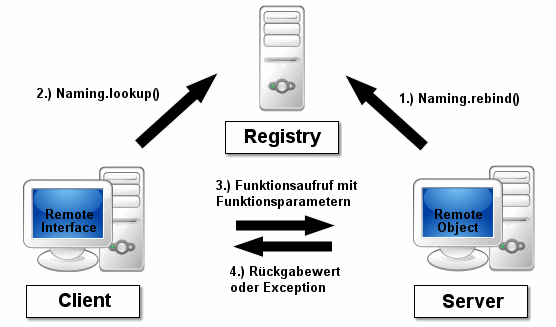
\includegraphics[scale=0.35]{images/rmi-schema.png}%
\end{wrapfigure}
Der Ablauf bei RMI:
\begin{enumerate}
	\item Der Server registriert ein Remote Object bei der RMI-Registry unter einem eindeutigen Namen.
	\item Der Client sieht bei der RMI-Registry unter diesem Namen nach und bekommt eine Objektreferenz, die seinem Remote Interface entsprechen muss.
	\item Der Client ruft eine Methode aus der Objektreferenz auf. Dabei kann ein Objekt einer Klasse X übergeben werden, die der JVM des Servers bisher nicht bekannt ist. In diesem Fall lädt die Server-JVM die Klasse X dynamisch nach, beispielsweise vom Webserver des Client.
	\item Die Server-JVM führt die Methode auf dem Remote Object aus, wobei evtl. dynamisch geladener Fremdcode benutzt wird, der im Allgemeinen Sicherheitsrestriktionen unterliegt. Dem Client werden die Rückgabewerte dieses Aufrufes gesendet, oder der Client bekommt eine Fehlermeldung.
\end{enumerate}
\subsection{Naming / Registry}
\begin{description}
	\item[bind] (String, Remote)\hfill 
		\begin{itemize}
			\item {\color{red} can only be called on localhost}
			\item Binds a specified name to a remote object
			\item May throw AlreadyBoundException
		\end{itemize}
	\item[rebind] (String, Remote)\hfill 
		\begin{itemize}
			\item {\color{red} can only be called on localhost}
			\item Rebinds a specified name to a remote object
		\end{itemize}
	\item[unbind] (String)\hfill 
		\begin{itemize}
			\item {\color{red} can only be called on localhost}
			\item Destroys the binding for a specified name
		\end{itemize}
	\item[lookup] (String)\hfill 
		\begin{itemize}
			\item Returns a reference to the remote object associated with the name
		\end{itemize}
	\item[list] (String)\hfill 
		\begin{itemize}
			\item Lists the names present in a registry
		\end{itemize}
\end{description}
\subsection{Using RMI}
\subsubsection{Remote Interfaces}
Define interfaces for remote classes:
\begin{itemize}
	\item All remotable interfaces must extend interface java.rmi.Remote
	\item All methods must throw a java.rmi.RemoteException
\end{itemize}
\begin{lstlisting}[language=Java, caption=Remote Interfaces, style=JavaStyle]
package ch.fhnw.ds.rmi.calculator;
public interface Calculator extends java.rmi.Remote {
   long add(long a, long b) throws java.rmi.RemoteException;
   long sub(long a, long b) throws java.rmi.RemoteException;
   long mul(long a, long b) throws java.rmi.RemoteException;
   long div(long a, long b) throws java.rmi.RemoteException;
}
\end{lstlisting}
\subsubsection{Implementation}
UnicastRemoteObject:
\begin{itemize}
	\item Implementation extends class Unicast- RemoteObject or calls explicitly UnicastRemoteObject.exportObject
	\item Implementation must implement the defined remote interface
\end{itemize}
\begin{lstlisting}[language=Java, caption=Implementation, style=JavaStyle]
package ch.fhnw.ds.rmi.calculator;
public class CalculatorImpl extends java.rmi.server.UnicastRemoteObject implements Calculator {
	public CalculatorImpl() throws java.rmi.RemoteException { }
	public long add(long a, long b) { return a + b; } 
	public long sub(long a, long b) { return a - b; } 
	public long mul(long a, long b) { return a * b; } 
	public long div(long a, long b) { return a / b; }
}
\end{lstlisting}
\subsubsection{stub and skeleton}
Create stub and skeleton classes using the rmic compiler:
\begin{itemize}
	\item No longer necessary in Java5 because Java5 adds support for the dynamic generation of stub classes at runtime
	\item rmic must still be used to pregenerate stub classes for remote objects that need to support clients running on earlier versions
	\item Dynamic Proxies
		\begin{itemize}
			\item Implemented using java.lang.reflect.Proxy
			\item Dynamic proxy is only used if no pregenerated stub class is available or if the system property java.rmi.server.ignoreStubClasses=true is set
			\item nly possible if clients run on Java 5 (or later)
		\end{itemize}
\end{itemize}
\subsubsection{Server}
Create and compile the server application (registration):
\begin{itemize}
	\item RMI service must be hosted in a server process
	\item RMI can use different naming services
\end{itemize}
\begin{lstlisting}[language=Java, caption=Server, style=JavaStyle]
package ch.fhnw.ds.rmi.calculator;
import java.rmi.Naming;
public class Server {
public static void main(String args[]) throws Exception {
      Calculator c = new CalculatorImpl();
      Naming.rebind("CalculatorService", c);
   }
}
\end{lstlisting}
\subsubsection{Client}
Create and compile a client program to access the remote objects:
\begin{lstlisting}[language=Java, caption=Client, style=JavaStyle]
package ch.fhnw.ds.rmi.calculator;
import java.rmi.Naming;
public class CalculatorClient {
	public static void main(String[] args) throws Exception {
    		Calculator c = (Calculator)Naming.lookup("rmi://localhost/CalculatorService");
		System.out.println( c.sub(4, 3) ); 
		System.out.println( c.add(4, 5) ); 
		System.out.println( c.mul(3, 6) ); 
		System.out.println( c.div(9, 3) );
	}
}
\end{lstlisting}
\subsubsection{Start of RMI-Registry \& Server}
\begin{lstlisting}[language=Java, caption=Example Variant, style=JavaStyle]
package ch.fhnw.ds.rmi.calculator;
public class Server {
   public static void main(String args[]) throws Exception {
		try {
			LocateRegistry.createRegistry(1099);
      	} catch (RemoteException e) {
			System.out.println(">> registry could not be exported");
			System.out.println(">> probably another registry already runs on 1099");
		}
      	Calculator c = new CalculatorImpl(0x7777);
		Naming.rebind("rmi://localhost:1099/CalculatorService", c);
		System.out.println("Calculator server started...");
	}
}
\end{lstlisting}
\begin{lstlisting}[language=Java, caption=List of all registered objects, style=JavaStyle]
public class ListRMIRegistry {
   public static void main(String[] args) throws Exception {
      if (args.length>0) {
         String host = args[0];
         if(args.length>1){
			host = host + ":" + Integer.parseInt(args[1]);
		 }
         String s[] = Naming.list("rmi://"+host);
         for(int i=0; i<s.length; i++) System.out.println(s[i]);
	  } else {
         System.out.println("Usage: java ListRMIREgistry " + "<host> [<port>]");
	  }
  }
}
\end{lstlisting}
\subsection{Marshalling}
Transfer of parameters to remote object (input or output):
\begin{description}
	\item[Parameters of primitive type] (int, double, ...) \hfill \\
		passed by value, in a machine-independent format
	\item[Parameters which are Serializable] (e.g. String) \hfill \\
		serializable objects are copied $\Ra$ call by value
	\item[Parameters which are Remote] \hfill \\
		only the reference to the remote object is passed, i.e. a new proxy is generated $\Ra$ call by reference
	\item[Parameters which are neither Serializable nor Remote] \hfill \\
		cannot be transferred (checked at runtime)
\end{description}
\begin{lstlisting}[language=Java, caption=QuoteServer, style=JavaStyle]
public void addQuoteListener(QuoteListener c) {
   synchronized (clients) { clients.add(c); }
}
\end{lstlisting}
\begin{lstlisting}[language=Java, caption=QuoteClient, style=JavaStyle]
QuoteServer server = (QuoteServer)Naming.lookup("rmi://localhost/QuoteServer");
server.addQuoteListener(new AbstractQuoteListener() {
	public void update(String s) {
		System.out.println(s);
	}
});
\end{lstlisting}
\subsection{Export / Unexport}
UnicastRemoteObject:
\begin{description}
	\item[Remote exportObject(Remote obj, int port)] \hfill
		\begin{itemize}
			\item Exports remote object
			\item Makes it available to receive remote calls
			\item Returns the remote object stub
		\end{itemize}
	\item[boolean unexportObject(Remote obj, boolean force)] \hfill
		\begin{itemize}
			\item Removes remote object from the RMI runtime
			\item If force==false, object is only unexported if no calls are in progress or pending
			\item Returns true if operation is successful, false otherwise
		\end{itemize}
\end{description}
\begin{lstlisting}[language=Java, caption=Example Interface, style=JavaStyle]
public interface Counter extends Remote {
	public int getValue() throws RemoteException(); 
	public int increment() throws RemoteException; 
	public int reset() throws RemoteException;
	// copies instance to a server 
	public Counter migrateTo(String host) throws RemoteException; 
	// copies counter back to the caller
	public Counter migrateBack() throws RemoteException; 
}
\end{lstlisting}
\begin{lstlisting}[language=Java, caption=Migrator interface, style=JavaStyle]
public interface Migrator extends Remote {
	public Counter migrate(Counter counter) throws RemoteException;
}
\end{lstlisting}
\begin{lstlisting}[language=Java, caption=Migrator implementation, style=JavaStyle]
public class MigratorImpl extends UnicastRemoteObject implements Migrator {
	public MigratorImpl() throws RemoteException { }
	public Counter migrate(Counter counter) throws RemoteException {
		UnicastRemoteObject.exportObject(counter, 0);
		return counter; // Variant: return the proxy
	}
}
\end{lstlisting}
\begin{lstlisting}[language=Java, caption=Counter implementation, style=JavaStyle]
public class CounterImpl implements Counter, Serializable { 
	private int value;
	public int getValue() { return value; }
	public int increment() { value++; return value; } 
	public int reset() { value = 0; return value; }
	public Counter migrateTo(String host) throws RemoteException {
		try {
			Migrator migrator = (Migrator) Naming.lookup("rmi://" + host + "/Migrator");
			return migrator.migrate(this);
		} catch(Exception e) { throw new RuntimeException(e); }
	}
	public Counter migrateBack() throws RemoteException {
		UnicastRemoteObject.unexportObject(this, true); 
		return this;
	}
}
\end{lstlisting}
\subsection{Threads}
\subsubsection{Specification}
A method dispatched by the RMI runtime to a remote object implemen- tation may or may not execute in a separate thread. The RMI runtime makes no guarantees with respect to mapping remote object invocations to threads. Since remote method invocation on the same remote object may execute concurrently, a remote object implementation needs to make sure its implementation is thread-safe \\
\subsubsection{Consequence}
\begin{itemize}
	\item You have to assume that your objects are called from different threads
	\item You have to implement objects thread-safe
\end{itemize}
\subsection{Dynamically Loaded Classes}
\begin{description}
	\item[Required classes can be loaded over the network] \hfill \\
		E.g. provided by a webserver
	\item[Class Loading / Security] \hfill
		\begin{itemize}
			\item A special class loader is provided: RMIClassLoader
			\item Security manager has to support remote class loading \\
				System.setSecurityManager(new RMISecurityManager())
		\end{itemize}
	\item[Start of RMI-Registry] \hfill
		\begin{itemize}
			\item rmiregistry must not contain the needed classes in its path!!
			\item Specify the java.rmi.server.useCodebaseOnly=false option (since Java7) \\
				rmiregistry -J-Djava.rmi.server.useCodebaseOnly=false
		\end{itemize}
	\item[Start of Server] \hfill
		\begin{itemize}
			\item Specify codebase for downloading class files
			\item java -Djava.rmi.server.codebase=http://localhost:8080 ch.fhnw.ds.rmi.calculator.Server
		\end{itemize}
	\item[Start of Client] \hfill
		\begin{itemize}
			\item permission to access server has to be provided (due to security manager)	\\
				java -Djava.security.policy=policy.txt ch.fhnw.ds.rmi.calculator.Client localhost
			\item policy file \\
				grant \{ permission java.net.SocketPermission "10.223.240.137:1024-",  "connect,resolve"; \}; 
		\end{itemize}
\end{description}
\subsection{Socket Factories}
\begin{description}
	\item[RMI Servers] \hfill
		\begin{itemize}
			\item When RMI object is exported, then a ServerSocket is created
			\item Access to a RMI object is established over a Socket
			\item Several objects may be exported over the same ServerSocket
		\end{itemize}
	\item[Socket Factories] \hfill
		\begin{itemize}
			\item Provide your own ServerSockets and Sockets to RMI
			\item Applications \\
				Authentication, Encryption, Compression, HTTP tunneling, time-out control
			\item Factories	\\
				ServerSocketFactory (returns ServerSocket), ClientSocketFacotory (returns Socket, is downloaded to client)
			\item Specified with exportObject
		\end{itemize}
\end{description}
\subsection{Example: XOR encoding}
\begin{center}
	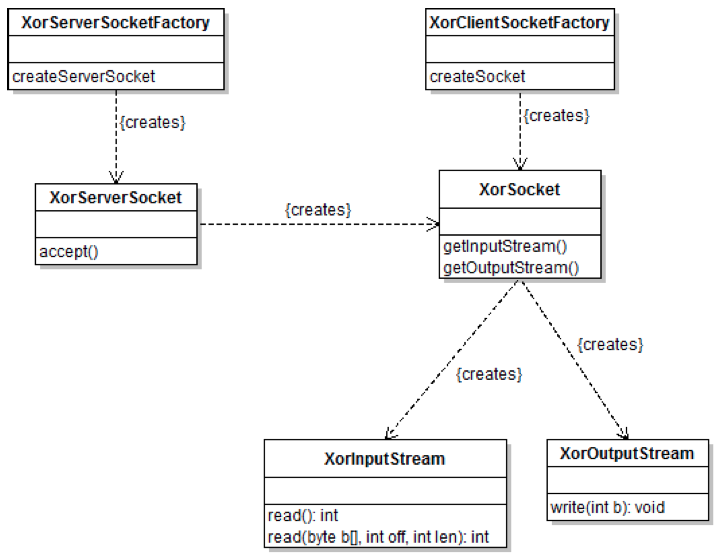
\includegraphics[scale=0.3]{images/rmi-factory.png}
\end{center}
\begin{lstlisting}[language=Java, caption=XorServerSocketFactory, style=JavaStyle]
public class XorServerSocketFactory implements RMIServerSocketFactory {
	private final byte pattern;
	public XorServerSocketFactory(byte pat) {this.pattern = pat;}
	public ServerSocket createServerSocket(int port) throws IOException {
		return new XorServerSocket(port, pattern);
	}
	public int hashCode() { return (int) pattern; }
	public boolean equals(Object obj) {
		return obj != null && getClass() == obj.getClass() && pattern == ((XorServerSocketFactory)obj).pattern);
	}
}
\end{lstlisting}
\begin{lstlisting}[language=Java, caption=XorClientSocketFactory, style=JavaStyle]
public class XorClientSocketFactory implements RMIClientSocketFactory, Serializable {
	private final byte pattern;
	public XorClientSocketFactory(byte pat) {this.pattern = pat;}
	public Socket createSocket(String host, int port) throws IOException {
		return new XorSocket(host, port, pattern);
	}
	public int hashCode() {return (int) pattern;}
	public boolean equals(Object obj) {
	return obj != null && getClass() == obj.getClass() && pattern == ((XorClientSocketFactory) obj).pattern;
	}
}
\end{lstlisting}
\begin{lstlisting}[language=Java, caption=XorServerSocket, style=JavaStyle]
class XorServerSocket extends ServerSocket { private final byte pattern;
	public XorServerSocket(int port, byte pattern) throws IOException {
		super(port); this.pattern = pattern;
	}
	public Socket accept() throws IOException {
		Socket s = new XorSocket(pattern); implAccept(s); return s;
	}
}
\end{lstlisting}
\begin{lstlisting}[language=Java, caption=XorSocket, style=JavaStyle]
class XorSocket extends Socket { 
	private final byte pat;
	private InputStream in = null;
	private OutputStream out = null;
	public XorSocket(byte pat) throws IOException {
		super(); this.pat = pat;
	}
	public XorSocket(String host, int port, byte pat) throws IOException {
		super(host, port); this.pat = pat;
	}
	public synchronized InputStream getInputStream() throws IOException {
		if (in == null) 
			in  = new XorInputStream(super.getInputStream(), pat);
		return in;
	}
	public synchronized OutputStream getOutputStream() throws IOException {
    		if (out == null)
    			out = new XorOutputStream(super.getOutputStream(),pat);
		return out;
	}
}
\end{lstlisting}
\begin{lstlisting}[language=Java, caption=XorOutputStream, style=JavaStyle]
class XorOutputStream extends FilterOutputStream { private final byte pattern;
	public XorOutputStream(OutputStream out, byte pattern) {
		super(out); this.pattern = pattern;
	}
	public void write(int b) throws IOException { 
		out.write((b ^ pattern) & 0xFF);
	}
}
\end{lstlisting}
\begin{lstlisting}[language=Java, caption=XorOutputStream, style=JavaStyle]
class XorInputStream extends FilterInputStream {
	private final byte pattern;
	public XorInputStream(InputStream in, byte pattern) {
		super(in); this.pattern = pattern;
	}
	public int read() throws IOException {
		int b = in.read();
		if (b != -1) // if not EOF or an error
      		b = (b ^ pattern) & 0xFF;
    		return b;
	}
	public int read(byte b[], int off, int len) throws IOException {
		int numBytes = in.read(b, off, len);
		for (int i = 0; i < numBytes; i++) {
			b[off + i] = (byte) ((b[off + i] ^ pattern) & 0xFF);
		return numBytes;
	}
}
\end{lstlisting}
\begin{lstlisting}[language=Java, caption=Use XorFactories, style=JavaStyle]
public class CalculatorImpl extends java.rmi.server.UnicastRemoteObject implements rmi.calculator.Calculator {
	public CalculatorImpl(int port) throws java.rmi.RemoteException{
		this(port, (byte)0xAC);
  	}
	public CalculatorImpl(int port, byte pat) throws java.rmi.RemoteException {
		super(port, new XorClientSocketFactory(pat), new XorServerSocketFactory(pat));
	}
	public long add(long a, long b) { return a + b; } 
	public long sub(long a, long b) { return a - b; } 
	public long mul(long a, long b) { return a * b; } 
	public long div(long a, long b) { return a / b; }
}
\end{lstlisting}

\newpage
\section{Asynchronous Communication}
\subsection{Prinzip}
\subsubsection{Synchronous Communication Model}
Client and Server are directly coupled (Telephone Connection)
\begin{center}
	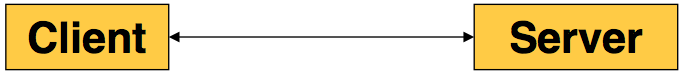
\includegraphics[scale=0.25]{images/communication-synchron.png}
\end{center}
\subsubsection{Asynchronous Communication Model}
 Client and Server communicate over a 3rd party Message Oriented Middleware (MOM). (SMS, Email)
 \begin{center}
	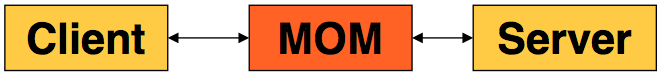
\includegraphics[scale=0.25]{images/communication-asynchron.png}
\end{center}
\subsection{Advantages}
\begin{itemize}
	\item Loosely coupled communication
	\item Sender/receiver do not have to be active at the same time and may be disconnected
	\item Sender/receiver only have to agree on message format, no dependency on interfaces
\end{itemize}
\subsection{Model}
\begin{itemize}
	\item Producer sends a message to a virtual channel
	\item Producer does not have to wait for a reply
	\item Producer does not know who will receive the message
	\item Producer is not dependent on the availability of consumers
	\item Transaction and security context of a producer are not propagated to the consumer of a message
\end{itemize}

\newpage
\section{Java Message Service}
\subsection{Point-to-Point Messaging Domain}
\textbf{Queue:}
\begin{itemize}
	\item Every message is sent to a particular queue
	\item Consumer fetches message at a particular queue
	\item Message is kept until it is consumed/expired
\end{itemize}
\textbf{Characteristics:}
\begin{itemize}
	\item Each message is consumed by only one client
	\item No time dependency between sender and consumer
	\item Consumer acknowledges consumption of a message
	\item Queues are persistent
\end{itemize}
\subsection{Publish/Subscribe Messaging Domain}
\begin{center}
	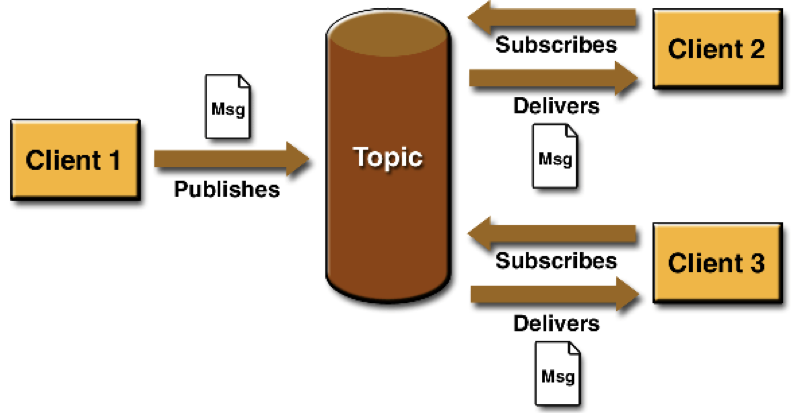
\includegraphics[scale=0.25]{images/jms-messaging-domain.png}
\end{center}
\textbf{Characteristics:}
\begin{itemize}
	\item Every message can be consumed by several clients
	\item Time dependency, only those messages are consumed which arrived after registration
	\item Consumer has to stay active
	\item A durable connection allows con- sumers to disconnect and later re- connect and collect messages that were published meanwhile
\end{itemize}
\subsection{Destinations}
\begin{tabular}{l p{2cm} l}
	\textbf{Queue} && \textbf{Topic} \\
	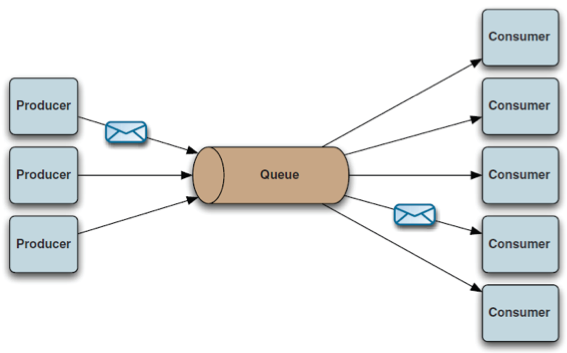
\includegraphics[scale=0.3]{images/jms-destination-queue.png} && 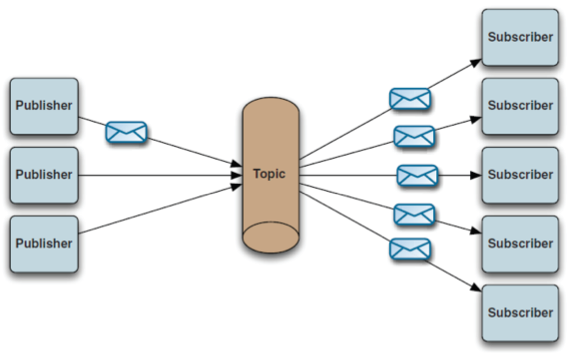
\includegraphics[scale=0.3]{images/jms-destination-topic.png} \\
	One-to-one message paradigm && One-to-many message paradigm	
\end{tabular}
\subsection{Message Consumption}
\begin{description}
	\item[Synchronously] \hfill \\
		JMS Client can receive messages explicitly
		\begin{itemize}
			\item[blocking mode] receive()
			\item[time-out mode] receive(int timeout)
		\end{itemize}
	\item[Asynchronously] \hfill \\
		JMS Client can register a message listener which is invoked when a message arrives \\
		setMessageListener()
\end{description}
\subsection{JMS API}
\subsubsection{Overview}
\begin{center}
	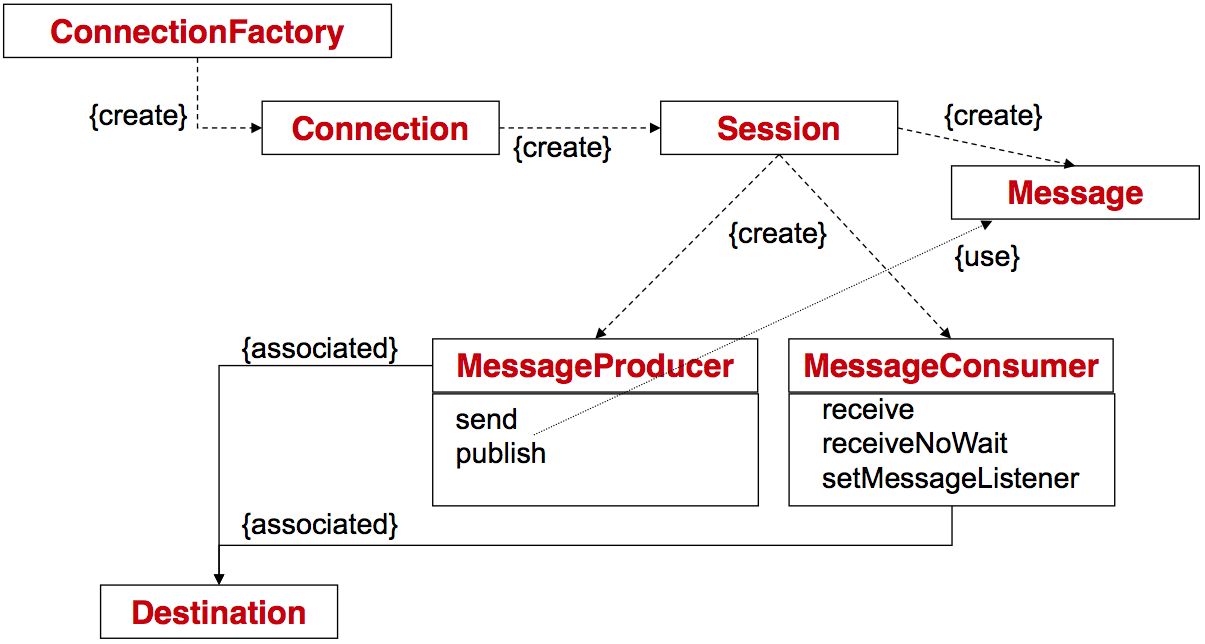
\includegraphics[scale=0.25]{images/jms-api-overview.png}
\end{center}
\subsubsection{Destinations}
\begin{wrapfigure}{r}{4cm}
	\centering
	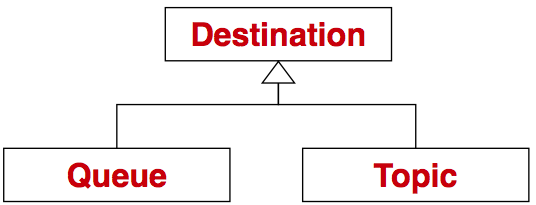
\includegraphics[scale=0.2]{images/jms-api-destination.png}%
\end{wrapfigure}
Destinations:
\begin{itemize}
	\item Destination where messages are delivered to or received from
		\begin{description}
			\item[Queue] point-to-point messaging domain destination
			\item[Topic] publish/subscribe messaging domain destination
		\end{description}
	\item A JMS application can work with several destinations
	\item New destinations are created using an administration tool
	\item Destinations are accessed using JNDI
\end{itemize}


\subsubsection{Connections}
\begin{wrapfigure}{r}{4cm}
	\centering
	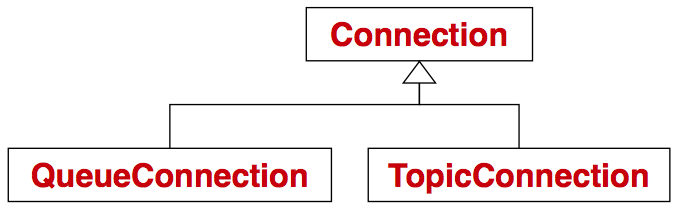
\includegraphics[scale=0.2]{images/jms-api-connection.png}%
\end{wrapfigure}
Connections:
\begin{itemize}
	\item Represents a communication channel to the JMS provider
	\item Connection has to be started before use (before receiving messages)
	\item Connection has to be closed when the program is done using it
\end{itemize}
\textbf{Connection Factories:}
\begin{itemize}
	\item Connections are created from connection factories
	\item Factories are accessed via JNDI	
	\item Java EE: two factories preconfigured
\end{itemize}
\textbf{Connection.start:}
\begin{itemize}
	\item Until connection is started, message flow does not occur
	\item Connection has to be started before messages can be transmitted or received
\end{itemize}
\textbf{Connection.close:}
\begin{itemize}
	\item Clients should close a connection as a provider typically allocates significant resources outside the JVM on behalf of a connection
	\item There is no need to close the sessions, producers, and consumers of a closed connection
	\item Closing a connection causes all temporary destinations to be deleted
\end{itemize}
\subsubsection{Sessions}
\begin{wrapfigure}{r}{4cm}
	\centering
	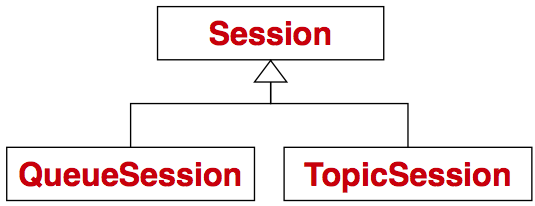
\includegraphics[scale=0.2]{images/jms-api-session.png}%
\end{wrapfigure}
Sessions:
\begin{itemize}
	\item Single-threaded context to deliver and consume message \\
		Any message sending and receiving happens in a serial order, one-by-one
	\item Transactional \\
		A set of send and receive operations can be packed in an atomic operation
	\item Sessions are created from connections \\
		createQueueSession(boolean transacted, int acknowledgeMode)	 \\
		createTopicSession(boolean transacted, int acknowledgeMode)
\end{itemize}

\subsubsection{Message Producers}
\begin{wrapfigure}{r}{4cm}
	\centering
	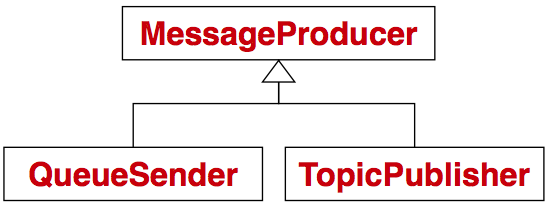
\includegraphics[scale=0.2]{images/jms-api-message-producer.png}%
\end{wrapfigure}
Message Producers:
\begin{itemize}
	\item Used to send or publish message
	\item TCreated from session object (createSender / createPublisher)
	\item Producer is associated with a destination (queue or topic) \\
		queueSession.createSender(queue)	 \\
		topicSession.createPublisher(topic) 
	\item Delivery of message with send / publish
\end{itemize}

\subsubsection{Message Consumers}
\begin{wrapfigure}{r}{4cm}
	\centering
	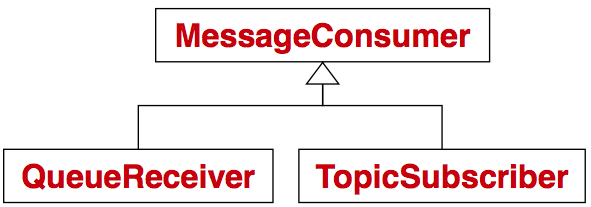
\includegraphics[scale=0.2]{images/jms-api-message-consumer.png}%
\end{wrapfigure}
Message Consumers:
\begin{itemize}
	\item Used to receive messages
	\item Created from session object (createReceiver / createSubscriber)
	\item Consumer is associated with a destination (queue or topic)
	\item Receipt of message with receive()/receiveNoWait()
	\item Deactivation with close()
	\item Messages are received after the connection is started
	\item Message filter can be specified for message consumers
\end{itemize}
\subsubsection{Message Listeners}
\begin{itemize}
	\item comparable to event listener (interface MessageListener \{ void onMessage(Message msg); \})
	\item Can be registered both in a QueueReceiver and a TopicSubscriber
	\item Per session only one listener is active
\end{itemize}
\subsubsection{Messages}
\begin{wrapfigure}{r}{8cm}
	\centering
	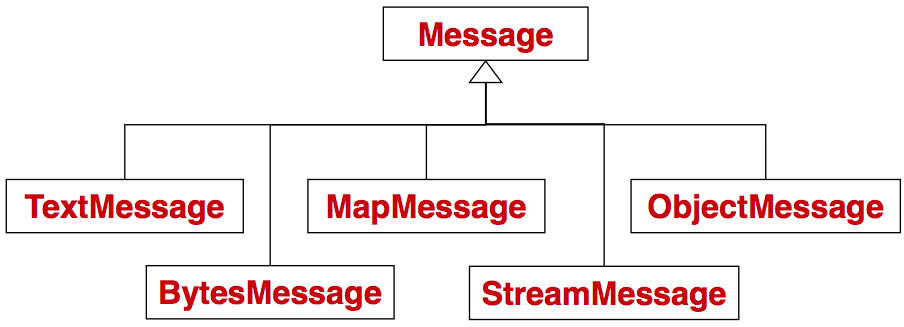
\includegraphics[scale=0.2]{images/jms-api-message.png}%
\end{wrapfigure}
Message Parts:
\begin{itemize}
	\item Header
	\item Properties [optional]
	\item Body [optional]
\end{itemize}
\textbf{Header Fields:} \\ \\
\begin{tabular}{l l l l}
	JMSDestination & send/publish \\
	JSMDeliveryMode & send/publish & int & persistency \\
	JMSExpiration & send/publish & long & time() + TTL msec \\
	JMSPriority & send/publish & int & 0 (low) .. 9 (high) \\
	JMSMessageID & send/publish \\
	JMSTimestamp & send/publish \\
	JMSCorrelationID & client \\
	JMSReplyTo & client \\
	JMSType	 & client & String \\
	JMSRedelivered & JMS provider \\
\end{tabular} \\ \\ \\
\textbf{Properties: }
\begin{itemize}
	\item additional properties can be specified by client (String/primitive - pairs)
\end{itemize}
\textbf{Body depends on message type:}
\begin{description}
	\item[TextMessage] String (getText/setText)
	\item[MapMessage] set of name/value pairs (String/primitive)
	\item[BytesMessage] byte stream
	\item[StreamMessage] sequence of primitive data types
	\item[ObjectMessage] contains one serializable object
	\item messages are created over a session object, there exist 5 factory methods:
		\begin{itemize}
			\item TextMessage m = session.createTextMessage();
			\item MapMessage m = session.createMapMessage();
			\item BytesMessage m = session.createBytesMssage();
			\item StreamMessage m = session.createStreamMessage();
			\item ObjectMessage m = session.createObjectMessage();
		\end{itemize}
\end{description}
\subsection{Sending / Receiving a Message}
\begin{enumerate}
	\item Obtain a connection factory that provides JMS connections to the messaging system
	\item Obtain a topic or a queue that represents a destination address for the message
	\item Create an connection to the JMS provider using the factory
	\item Create a session that is used to group the actions of sending and receiving messages (single-threaded context)
	\item Create a publisher or a sender that sends messages to the specified topic or queue
	\item create a subscriber or a receiver and optionally register a MessageListener that receives messages from the specified topic or queue
\end{enumerate}
\subsection{Examples}
\subsubsection{Simple Example}
\begin{lstlisting}[language=Java, caption=Simple Example Sender, style=JavaStyle]
public class SimpleQueueSender {
	public static void main(String[] args) throws Exception {
		Context jndiContext = new InitialContext(); 
		QueueConnectionFactory queueConnectionFactory = (QueueConnectionFactory) jndiContext.lookup("QueueConnectionFactory");
		Queue queue = (Queue) jndiContext.lookup(args[0]);
		QueueConnection qconn = null;
		try {
			qconn = queueConnectionFactory.createQueueConnection(); 
			QueueSession queueSession = qconn.createQueueSession(false, Session.AUTO_ACKNOWLEDGE);
			QueueSender queueSender=queueSession.createSender(queue);
			TextMessage m = queueSession.createTextMessage();
			for (int i = 0; i < 3; i++) {
				m.setText("This is message " + (i + 1));
				queueSender.send(m);
			}
		} finally {
			if (qconn != null)
				try { qconn.close(); } catch(JMSException e){}
		}
	}
}
\end{lstlisting}
\begin{lstlisting}[language=Java, caption=Simple Example Receiver, style=JavaStyle]
public class SimpleQueueReceiver {
	public static void main(String[] args)  throws Exception {
		Context jndiContext = new InitialContext();
		QueueConnectionFactory queueConnectionFactory = (QueueConnectionFactory) jndiContext.lookup("QueueConnectionFactory");
		Queue queue = (Queue) jndiContext.lookup(args[0]);
		QueueConnection qConn = null;
		try {
			qConn = queueConnectionFactory.createQueueConnection(); 
			QueueSession queueSession = qConn.createQueueSession(false, Session.AUTO_ACKNOWLEDGE);
			QueueReceiver queueReceiver = queueSession.createReceiver(queue);
			qConn.start(); 
			while (true) {
				Message m = queueReceiver.receive();
				if (m instanceof TextMessage) {
					TextMessage message = (TextMessage) m;
					System.out.println("Reading message: " + message.getText());
				}
			}
		} finally {
			if (qConn != null)
				try {qConn.close();} catch (JMSException e) {}
		}
	}
}
\end{lstlisting}
\subsubsection{Echo}
\begin{lstlisting}[language=Java, caption=Echo Client, style=JavaStyle]
public static void main(String[] args) throws Exception{ 
	Hashtable<String,String> properties = new Hashtable<String,String>();
  ...
	Context context = new InitialContext(properties);
	QueueConnectionFactory factory = (QueueConnectionFactory) context.lookup("ConnectionFactory");
	Queue queue = (Queue) context.lookup("ECHO");
	QueueConnection connection=factory.createQueueConnection("","");
	QueueSession session = connection.createQueueSession(false, QueueSession.AUTO_ACKNOWLEDGE);
	QueueSender sender  = session.createSender(queue);
	TemporaryQueue tempQueue = session.createTemporaryQueue();
	QueueReceiver receiver = session.createReceiver(tempQueue);
	connection.start();
	TextMessage request = session.createTextMessage(); 
	request.setText("Hello World [" + new Date() + "]");
	request.setJMSReplyTo(tempQueue); sender.send(request);
	TextMessage response = (TextMessage) receiver.receive();
	System.out.println("Response: " + response.getText());
	connection.close();
}
\end{lstlisting}
\begin{lstlisting}[language=Java, caption=Echo Server, style=JavaStyle]
public static void main(String[] args) throws Exception{ 
	Hashtable<String,String> properties = new Hashtable<String,String>();
   ...
	Context context = new InitialContext(properties);
	QueueConnectionFactory factory = (QueueConnectionFactory) context.lookup("ConnectionFactory");
	Queue queue = (Queue) context.lookup("ECHO");
	QueueConnection connection=factory.createQueueConnection("","");
	QueueSession session = connection.createQueueSession(false, QueueSession.AUTO_ACKNOWLEDGE);
	QueueReceiver receiver = session.createReceiver(queue); 
	connection.start();
	System.out.println("Echo service is running..."); 
	while(true){
		TextMessage request = (TextMessage)receiver.receive();
		Queue replyQueue = (Queue) request.getJMSReplyTo(); 
		TextMessage response = session.createTextMessage(); 
		response.setText("Echo: "+request.getText()); 
		QueueSender sender = session.createSender(replyQueue); 
		sender.send(response);
		System.out.println("Handled "+request.getText());
	}
}
\end{lstlisting}
\subsection{Guaranteed Messaging and Transactions}
\subsubsection{Delivery Mode}
\begin{description}
	\item[PERSISTENT] (Default)\hfill \\
		Instructs the JMS provider to take extra care to ensure that message is not lost in case of a JMS provider failure
	\item[NON\_PERSISTENT] \hfill \\
		Does not require the JMS provider to store the message
\end{description}
\subsubsection{Specification of delivery mode:}
\begin{description}
	\item[On MessageProducer] \hfill \\
		producer.setDeliveryMode(DeliveryMode.NON\_PERSISTENT)
	\item[On send or publish method] \hfill \\
		producer.send(msg, DeliveryMode.NON\_PERSISTENT, 4, 10000)
		\begin{itemize}
			\item Priority level: 0 (lowest), 4 (default), 9 (highest)
			\item Message expiration in msec
		\end{itemize}
\end{description}
\subsubsection{Durable Subscribers}
\begin{description}
	\item[Nondurable subscribers] \hfill \\
		Receive messages only when they are actively listening on a topic
	\item[Durable subscribers] \hfill
		\begin{itemize}
			\item Receive all messages sent to that topic (store-and-forward messaging)
			\item Messages are stored under a subscriber ID (ClientID-SubscriptionName)
			\item Durable subscribers must perform two initial steps:
				\begin{itemize}
					\item Set the ClientID on the connection (before creating any sessions).\\ The ClientID is part of the durable subscriber's name (a client can only be connected once)
					\item Use the createDurableSubscriber factory method of the topic session. This method requires a second parameter with the name of the durable subscriber
				\end{itemize}
			\item Durable subscribers may be unsubscribed
		\end{itemize}
\end{description}
\subsubsection{Message Acknowledgements}
\begin{itemize}
	\item Servers acknowledge the receipt of messages from producers
	\item Consumers acknowledge the receipt of messages from servers
\end{itemize}
\textbf{Modes:}
\begin{description}
	\item conn.createQueueSession(false, Session.CLIENT\_ACKNOWLEDGE);
	\item conn.createTopicSession(false, Session.CLIENT\_ACKNOWLEDGE);
	\item[AUTO\_ACKNOWLEDGE] \hfill \\
		Session automatically acknowledges receipt of a message
	\item[DUPS\_OK\_ACKNOWLEDGE] \hfill \\
		Same as AUTO, but messages may be delivered more than once
	\item[CLIENT\_ACKNOWLEDGE] \hfill
		\begin{itemize}
			\item Client acknowledges message by calling the message's acknowledge method
			\item Acknowledging a message acknowledges the receipt of ALL messages of that session
		\end{itemize}
\end{description}
\textbf{Duplicate Messages:}
\begin{itemize}
	\item With AUTO / DUPS\_OK acknowledgement modes acknowledgement may get lost
	\item To guard against duplicate messages an application must check whether a redelivered message was already processed
	\item JMSMessageId header is unique and can be used as a key in a table
\end{itemize}
\subsubsection{JMS Transactions}
\begin{itemize}
	\item conn.createQueueSession(true, Session. SESSION\_TRANSACTED);
	\item conn.createTopicSession(true, Session. SESSION\_TRANSACTED);
	\item All messages sent or received using such a session are automatically grouped in a transaction
	\item The transactioni remains open until either a session.rollback() or a session.commit() is invoked (which also starts a new transaction)
	\item Transactions guarantee
		\begin{itemize}
			\item That message is delivered from the client to the JMS provider
			\item That message is delivered from the JMS provider to the consumer
		\end{itemize}
\end{itemize}

\newpage
\section{WebSockets}
\subsection{Spec}
\subsubsection{Bidirectional Communication}
\begin{center}
	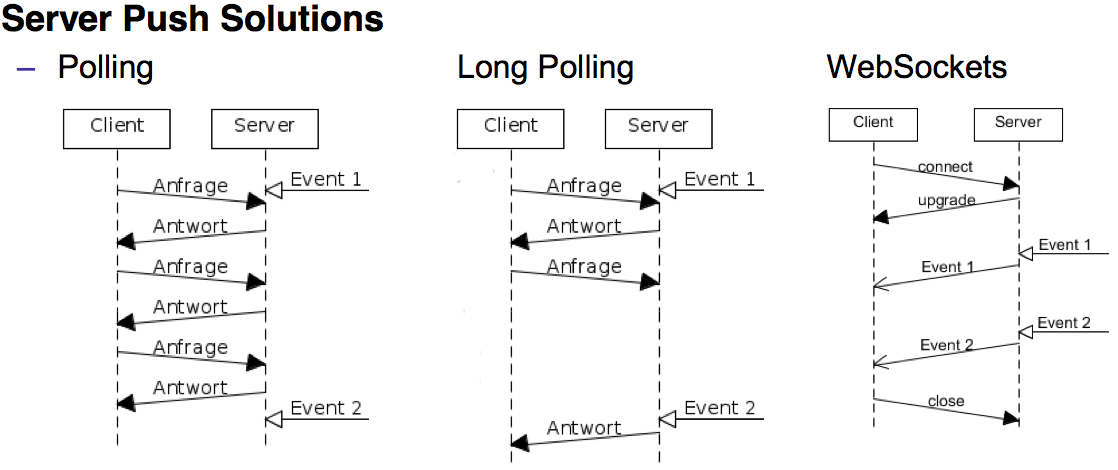
\includegraphics[scale=0.2]{images/websockets-server-push-solutions.png}
\end{center}
\subsubsection{Format}
\begin{center}
	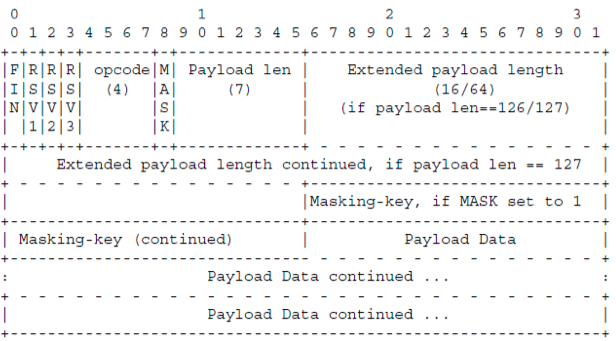
\includegraphics[scale=0.3]{images/websocket-spec-format.png}
\end{center}
\subsubsection{Handshake}
\begin{lstlisting}
GET /examples/websocket/echoStream HTTP/1.1 Host: server.example.com
Connection: Upgrade
Upgrade: websocket
Sec-Websocket-Key: mqn5Pm7wtXEX6BzqDInLjw==
Sec-Websocket-Version: 13
\end{lstlisting}
\begin{lstlisting}
HTTP/1.1 101 Switching Protocols
Server: Apache-Coyote/1.1
Upgrade: websocket
Connection: upgrade
Sec-WebSocket-Accept: +TdGPOkAq62+toDOhVGj2QZWwg8= Date: Thu, 04 Apr 2013 19:21:39 GMT
\end{lstlisting}
\subsubsection{Negotiation}
\begin{lstlisting}
GET /examples/websocket/echoStream HTTP/1.1 Host: server.example.com
Connection: Upgrade
Upgrade: websocket
Sec-Websocket-Key: mqn5Pm7wtXEX6BzqDInLjw==
Sec-WebSocket-Protocol: chat, superchat
Sec-Websocket-Version: 13
\end{lstlisting}
\begin{lstlisting}
HTTP/1.1 101 Switching Protocols
Server: Apache-Coyote/1.1
Upgrade: websocket
Connection: upgrade
Sec-WebSocket-Accept: +TdGPOkAq62+toDOhVGj2QZWwg8= Sec-WebSocket-Protocol: chat
Date: Thu, 04 Apr 2013 19:21:39 GMT
\end{lstlisting}
\subsection{Java-WebSocket}
\begin{lstlisting}[language=Java, caption=Echo Server, style=JavaStyle]
public class EchoServer extends WebSocketServer {
	public static void main(String[] args) {
		WebSocketServer server = new EchoServer(80);
		server.start();
	}
	public EchoServer( int port ) {
		super( new InetSocketAddress(port) );
	}
	public void onOpen(WebSocket c, ClientHandshake handshake) {
		System.out.println("onOpen " + c.getRemoteSocketAddress());
	}
	public void onClose(WebSocket c, int id, String s, boolean rem){
    		System.out.println("closed " + c.getRemoteSocketAddress());
  	}
	public void onMessage(WebSocket c, String message) {
		System.out.println("onMessage from" + c.getRemoteSocketAddress() + ": " + message );
		c.send("Echo: " + message);
	}
	public void onError(WebSocket c, Exception ex) {
		System.out.println("onError " + c + ":" + ex );
	}
}
\end{lstlisting}
\begin{lstlisting}[language=Java, caption=Echo Client, style=JavaStyle]
public class EchoClient {
	public static void main(String[] args) throws Exception {
		final URI url = new URI("ws://echo.websocket.org/");
		final WebSocketClient c = new WebSocketClient(url, new Draft_17()) {
			public void onOpen(ServerHandshake handshakedata) {
				System.out.println("onOpen");
				send("Hello");
			}
			public void onMessage(String message) {
        			System.out.println("onMessage "+message);
				close();
			}
			public void onError(Exception ex) {
				System.out.println("onError");
			}
			public void onClose(int code, String txt, boolean remote) {
				System.out.println("onClose");
			}
		};
    		c.connect();
	}
}
\end{lstlisting}
\subsubsection{Tomcat}
\begin{lstlisting}[language=Java, caption=Echo Server, style=JavaStyle]
public abstract class WebSocketServlet() {
	protected void doGet(HttpServletRequest req, HttpServletResponse resp) {...}
	protected abstract StreamInbound createWebSocketInbound( String subProtocol, HttpServletRequest request);
	protected String selectSubProtocol(List<String> subProtocols)
	protected boolean verifyOrigin(String origin)
}
public abstract class MessageInbound extends StreamInbound {
	protected abstract void onBinaryMessage(ByteBuffer message);
	protected abstract void onTextMessage(CharBuffer message);
	protected void onOpen(WsOutbound outbound) {} 
	protected void onClose(int status) {} 	
	protected void onPong(ByteBuffer payload) {}
}
public class EchoMessage extends WebSocketServlet {
	protected StreamInbound createWebSocketInbound(
		String subProtocol, HttpServletRequest request) {
			return new EchoMessageInbound();
		}
		private class EchoMessageInbound extends MessageInbound {
		protected void onBinaryMessage(ByteBuffer message) throws IOException {
			getWsOutbound().writeBinaryMessage(message);
    		}
    		protected void onTextMessage(CharBuffer message) throws IOException {
    			getWsOutbound().writeTextMessage(message);
		}
	}
}
\end{lstlisting}

\newpage
\section{Tuple Spaces}
\subsection{Prinzip}
\subsubsection{Distributed Shared Associative Memory Space}
\begin{itemize}
	\item Provides a repository of tuples that can be accessed concurrently \\
		Associative: items are selected by reference to their contents 
	\item Implements blackboard metaphor
		\begin{itemize}
			\item Producers post their data as tuples in the space
			\item Consumers retrieve data from the space that match a certain pattern
		\end{itemize}
\end{itemize}
\subsubsection{Uncoupling}
\begin{description}
	\item[Time:] Tuples have their own life span (independent of producers and consumers)
	\item[Destination:] The producer requires no knowledge about the future of a tuple, i.e. tuple space communication is fully anonymous
	\item[Space:] Tuple space provides a globally shared data space to all processes
\end{description}
\subsection{Overview}
\begin{itemize}
	\item Java implementation of the Linda coordination model
	\item Enables communication between applications in a network of heterogeneous computers and operating systems
	\item Features:
		\begin{itemize}
			\item Blocking and non-blocking tuple set operators
			\item Persistent data repository
			\item Database indexing and query capabilities
			\item Event notifications
			\item Access controls
		\end{itemize}
\end{itemize}
\subsection{Basic Definitions}
\subsubsection{Tuple	}
\begin{itemize}
	\item A tuple is an ordered sequence of fields
	\item Template tuple is a tuple used for matching
\end{itemize}
\subsubsection{Field}
\begin{itemize}
	\item Type	
	\item Value
	\item Name (optional) \\
		If a name is specified, then this field is indexed
\end{itemize}
\subsubsection{TupleSpace}
\begin{itemize}
	\item Implements a space where tuples can be added/removed
	\item It is stored and administered across a network on one or more "TSpace Servers" (a TSpace server may contain many TupleSpaces)
	\item Several threads on the same or different machines can be accessing the space simultaneously
	\item For each different TupleSpace a client wishes to access, it requires a separate instance of this class, even if they are managed by the same server
	\item In order to obtain an instance of a specific tuple space you need the name of the space, and the name of a server that manages that space (and a port)
\end{itemize}
\begin{lstlisting}[language=Java, caption=TupleSace, style=JavaStyle]
TupleSpace(String name, String host);
TupleSpace(String name, String host, int port);
\end{lstlisting}
\subsection{Primitive operations}
\begin{description}
	\item[write(Tuple tuple)] \hfill \\ Adds a tuple to the store
	\item[take(Tuple template)] non-blocking \hfill
		\begin{itemize}
			\item Searches for a tuple that matches the template
			\item When found, the tuple is removed from the space and returned
			\item If none is found, returns null
		\end{itemize}
	\item[waitToTake(Tuple template)] blocking \hfill \\
		Like take, but blocks until a match is found
	\item[read(Tuple template)] non-blocking \hfill \\
		 Like take, except that the tuple is not removed from the space
	\item[waitToRead(Tuple template)] blocking \hfill \\
		Like waitToTake, except that the tuple is not removed from the space
	\item[scan(Tuple template)] non-blocking \hfill
		\begin{itemize}
			\item Like read, except that it returns all tuples that match
			\item The tuples read are returned in one tuple (with the tuples as fields)	
		\end{itemize}
	\item[countN(Tuple template)] non-blocking \hfill
		\begin{itemize}
			\item Like scan, except that it returns the number of matching tuples only
			\item Not that useful as the number of tuples may have changed after invocation
		\end{itemize}
\end{description}
\subsection{Tuple}
\subsubsection{Ways to create a tuple}
\begin{lstlisting}[language=Java, caption=Ways to create a tuple, style=JavaStyle]
Tuple t = new Tuple("key", "value");
Tuple t = new Tuple(); t.add("key"); t.add("value");
Tuple t = new Tuple(new Field("key"), new Field("value"));
Tuple t = new Tuple(new Field(String.class, "key"), "value");
Tuple t = new Tuple(new Field("key", String.class, "key"),new Field("value", String.class, "value"));
ts.write("key", "value");
\end{lstlisting}
\subsubsection{Ways to read a tuple}
\begin{itemize}
	\item  In order to read a tuple you must create a template Tuple
	\item A template Tuple is a Tuple that is used to select matching Tuples
	\item It will contain 0 or more fields that are either actual fields or formal fields
	\item Actual fields	\\
		have a value that must be matched exactly against the corresponding Fields in the tuples that are in the space
	\item Formal fields
		\begin{itemize}
			\item have a class but no value and only describe the type of value that is to be returned
			\item Basically they act as wildcards
		\end{itemize}
\end{itemize}
\begin{lstlisting}[language=Java, caption=Ways to read a tuple, style=JavaStyle]
Tuple template = new Tuple("key", "value"); Tuple t = ts.read(template);
Tuple template = new Tuple("key", new Field(String.class));
Tuple t = ts.read(template);
Tuple template = new Tuple(new Field(String.class),
                           new Field(String.class));
Tuple t = ts.read(template);
Tuple t = ts.read(new Field(String.class),
                  new Field(String.class));
\end{lstlisting}
\subsubsection{Echo Example}
\begin{lstlisting}[language=Java, caption=Echo Client, style=JavaStyle]
public class Client {
  public static void main(String[] args) throws Exception {
    TupleSpace ts = new TupleSpace("Echo", "localhost");
    UUID uuid = UUID.randomUUID();
    TupleID id = ts.write(new Tuple(uuid, "Hello World"));
    Tuple res = ts.waitToTake(new Tuple(new Field(String.class), uuid, new Field(String.class)));
    System.out.println(res.getField(2).getValue());
  }
}
\end{lstlisting}
\begin{lstlisting}[language=Java, caption=Echo Server, style=JavaStyle]
public class Server {
	public static void main(String[] args) throws Exception {
		TupleSpace ts = new TupleSpace("Echo", "localhost");
		while (true) {
    			Tuple template = ts.waitToTake(new Field(UUID.class), new Field(String.class));
			String text = (String) template.getField(1).getValue(); 
			ts.write(new Tuple("Response", template.getField(0), "Echo: " + text));
		}
	}
}
\end{lstlisting}
\subsubsection{Factorial Example}
\begin{lstlisting}[language=Java, caption=Master, style=JavaStyle]
public class Master {
	public static void main(String[] args) throws Exception {
		TupleSpace ts = new TupleSpace("Factorial", "localhost");
		ts.deleteAll();
		int n = 100;
		ts.write("counter", 1);
		for (int i = 0; i < n; i++) {
			ts.write("x", BigInteger.valueOf(i + 1));
			if (i > 0) ts.write("task");
		}
		Tuple res = ts.waitToTake(new Tuple("counter", n));
		res = ts.take(new Tuple("x", new Field(BigInteger.class)));
		System.out.println(n+"! = " + res.getField(1).getValue());
	}
}
\end{lstlisting}
\begin{lstlisting}[language=Java, caption=Worker, style=JavaStyle]
public class Worker {
	public static void main(String[] args) throws Exception {
		TupleSpace ts = new TupleSpace("Factorial", "localhost"); while (true) {
			ts.waitToTake("task");
			Tuple a1=ts.waitToTake("x", new Field(BigInteger.class));
			Tuple a2=ts.waitToTake("x", new Field(BigInteger.class)); 
			BigInteger x1 = (BigInteger) (a1.getField(1).getValue()); 
			BigInteger x2 = (BigInteger) (a2.getField(1).getValue()); 
			ts.write("x", x1.multiply(x2));
			Tuple c = ts.waitToTake("counter",new Field(Integer.class));
			ts.write("counter",(Integer) c.getField(1).getValue()+1);
		}
	}
}
\end{lstlisting}
\subsection{Transactions}
\begin{itemize}
	\item Create an instance of Transaction class
	\item Call method {\color{red}beginTrans} on the transaction
	\item Add a TupleSpace object to the transaction object using {\color{red}addSpace}
	\item Perform operations (write, read, ..) on the TupleSpace object added to the transaction
	\item Call {\color{red}commitTrans} on the transaction to make the effects of operations persistent
	\item Call {\color{red}abortTrans} method of Transaction object to undo all operations that belong to the current transaction
	\item A transaction may be added to several tuple spaces!
\end{itemize}
\begin{lstlisting}[language=Java, caption=Transaction Example, style=JavaStyle]
Transaction trans = new Transaction();
TupleSpace ts = new TupleSpace("testing");
trans.addSpace(ts);
trans.beginTrans(); // start of transaction 
ts.write("email", "to", "stefan.hoechli@fhnw.ch"); 
ts.write("email", "text", "Hello"); 
ts.write("email", "from", "dominik.gruntz@fhnw.ch"); 
trans.commitTrans(); // end of transaction
\end{lstlisting}
\subsection{Event Registration}
\subsubsection{Event notifications}
\begin{itemize}
	\item A mechanism that enables clients to register with the server in order to be informed when specific types of events are available
		\begin{itemize}
			\item WRITE
			\item DELETE
		\end{itemize}
	\item Event registration can be cancelled with eventDeRegister
\end{itemize}
\begin{lstlisting}[language=Java, caption=Event notifications Example, style=JavaStyle]
TupleSpace ts = new TupleSpace("testing");
Tuple template = new Tuple(new Field(String.class));
boolean newThread = false;
int id = ts.eventRegister("WRITE", template, callback, newThread);
...
ts.eventDeRegister(id);
\end{lstlisting}
\begin{lstlisting}[language=Java, caption=Callback interface, style=JavaStyle]
interface Callback {
	public boolean call(
		String commandName, 	// e.g. WRITE or DELETE
		String tsName, 				// the name of the tuple space this
                          // command was executed on.
		int sequenceNumber,		// the registration id for the
													// executed command
		SuperTuple tuple,			// the returned tuple or a tuple
													// which contains an exception boolean 
		isException 					// indicates whether the command
													// was processed normally or with
													// an exception
	);
}
\end{lstlisting}

\newpage
\section{Remoting Patterns}
\subsection{Remoting Styles}
\subsubsection{Remote Procedure Calls}
\begin{description}
	\item[Synchronous call] \hfill \\
		Client waits until invocation succeeds (asynchronous variants exist)
	\item[Remoting errors] \hfill \\
		In contrast to in-process operations remoting errors may occur
	\item[Procedure-RPC vs. OO-RPC] \hfill
		\begin{description}
			\item[Procedural:] \hfill
				\begin{itemize}
					\item  Server provides a set of operations
					\item Typically stateless services
				\end{itemize}
			\item[OO-RPC:] \hfill
				\begin{itemize}
					\item  Server hosts a set of objects $\Ra$ object identity
					\item Distributed object typically have their own state
 				\end{itemize}
		\end{description}
\end{description}
\subsubsection{Message Passing}
\begin{description}
	\item[Message Queue Service] \hfill
		\begin{itemize}
			\item Sender and Receiver decoupled by message queue servic
			\item Sender and receiver do not need to know each other
			\item Reliability
				\begin{itemize}
					\item Exactly-once-semantics for queues
					\item Acknowledgement of message consumption
				\end{itemize}
		\end{itemize}
	\item[Message Styles] \hfill
		\begin{itemize}
			\item Queue $\Ra$ one receiver
			\item Topic $\Ra$ many receivers 
		\end{itemize}
\end{description}
\begin{center}
	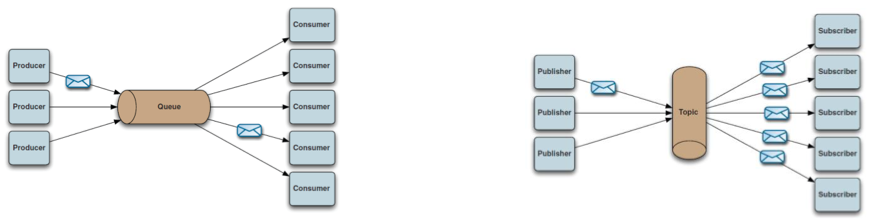
\includegraphics[scale=0.4]{images/remote-message-passing.png}
\end{center}
\subsubsection{Shared Repository}
\begin{itemize}
	\item Provides a small interface consisting of access primitives to the clients (CRUD)
	\item Idea based on (Linda's) Tuple Spaces
\end{itemize}
\textbf{Samples:} TupleSpaces, DataBases, REST
\subsection{Pattern Language for RPC-like communication}
\subsubsection{Pattern Language}
\begin{itemize}
	\item Collection of design patterns for a particular application domain
	\item Describes how to build a complex system of a certain type -- too complicated to be described in one pattern
	\item Patterns describe roles, need not necessarily form its own component, a component may play multiple roles at the same time
\end{itemize}
\subsubsection{Remote Object Access}
\textbf{Remote Object:}
\begin{itemize}
	\item Is accessed from client (over a well-defined interface) across machine boundary
	\item Has a unique object ID in its local address space
\end{itemize}
\begin{center}
	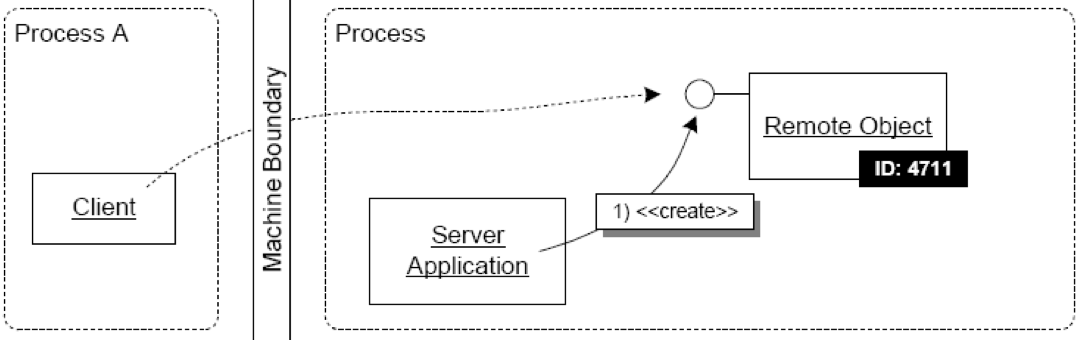
\includegraphics[scale=0.2]{images/remote-objects.png}
\end{center}
\textbf{Server Application:}
\begin{itemize}
	\item Creates and configures remote object
	\item Activates remote object and makes it available to remote clients
	\item Publishes remote object in a naming service
	\item Destroys remote instances not needed anymore
\end{itemize}
\begin{center}
	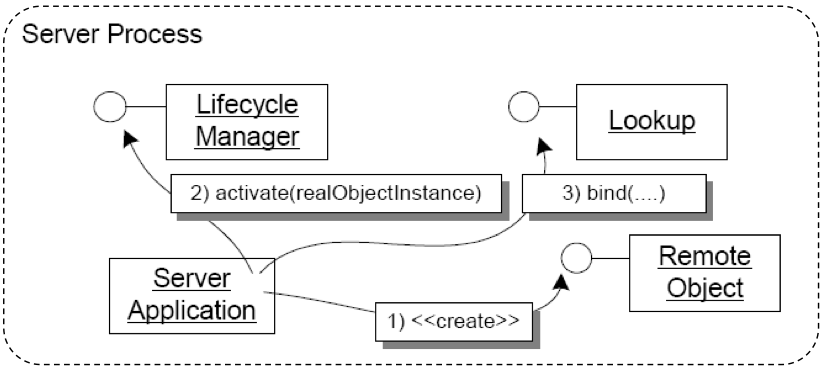
\includegraphics[scale=0.2]{images/server-application.png}
\end{center}
\subsection{Basic Remoting Patterns}
\subsubsection{Overview}
\begin{center}
	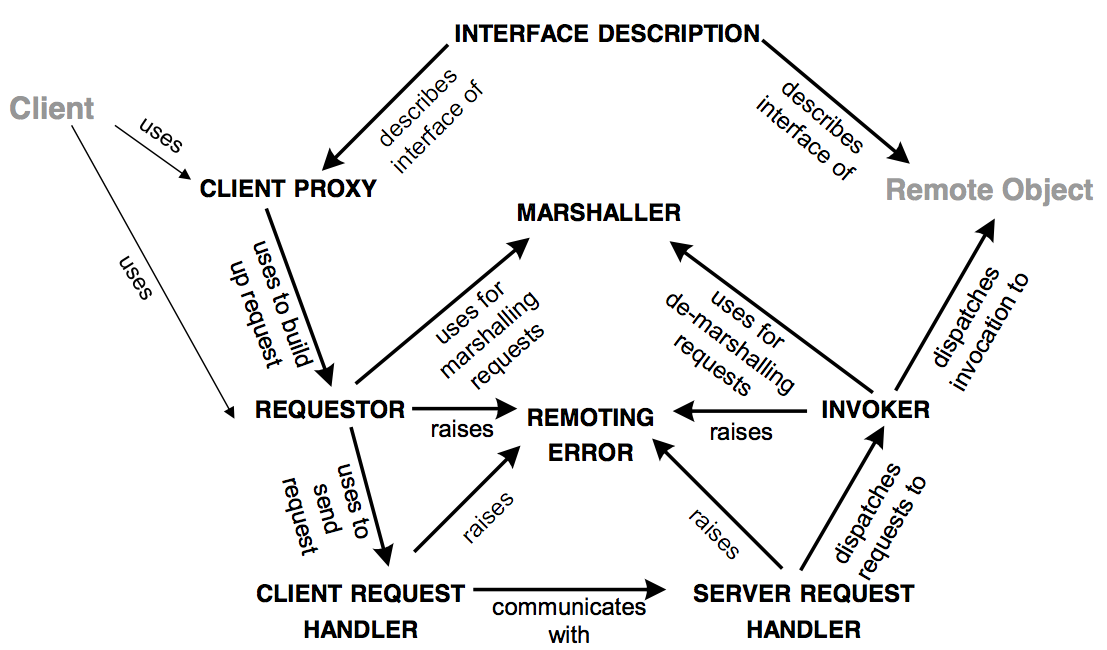
\includegraphics[scale=0.25]{images/basic-remote-patterns.png}
\end{center}
\subsubsection{Interactions}
\begin{center}
	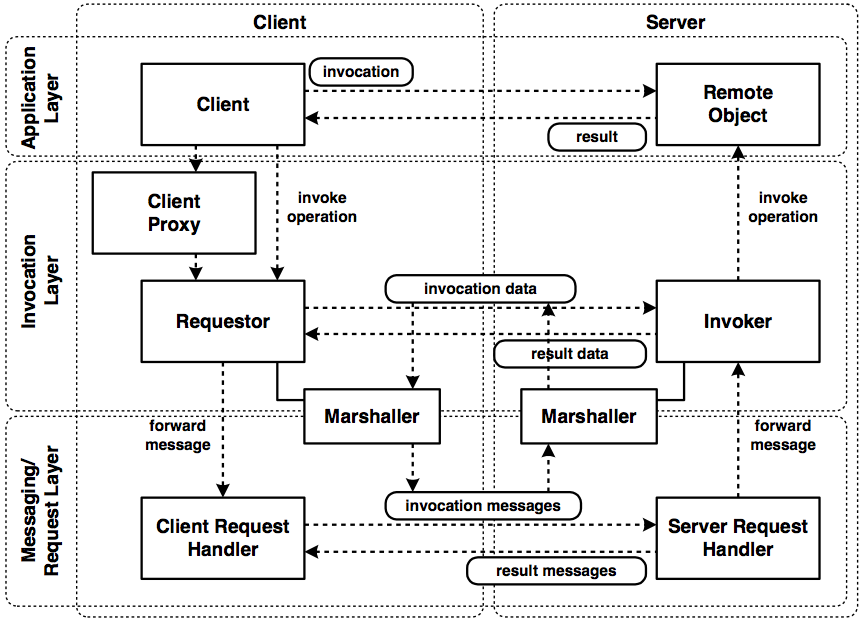
\includegraphics[scale=0.25]{images/interactions.png}
\end{center}
\textbf{Basic invocation sequence on client side:}
\begin{center}
	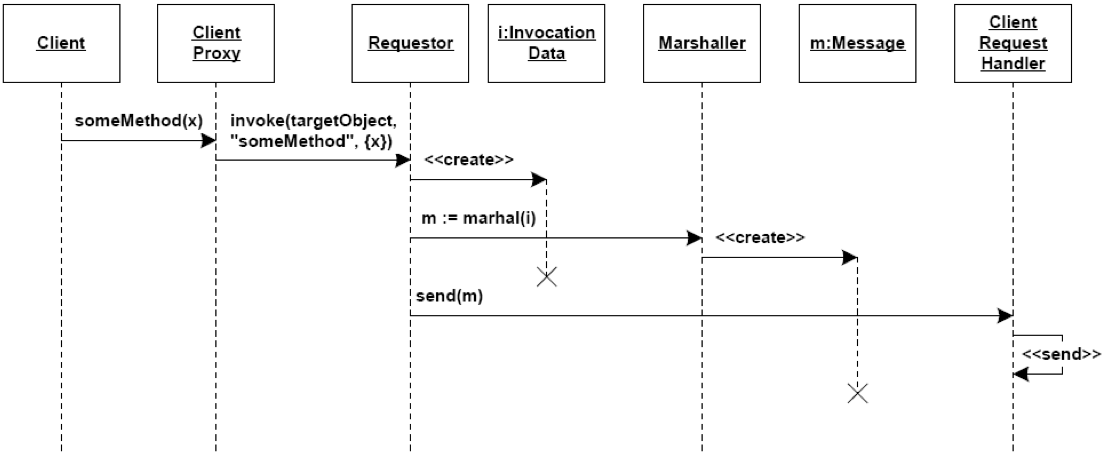
\includegraphics[scale=0.25]{images/invocation-client.png}
\end{center}
\textbf{Basic invocation sequence on server side:}
\begin{center}
	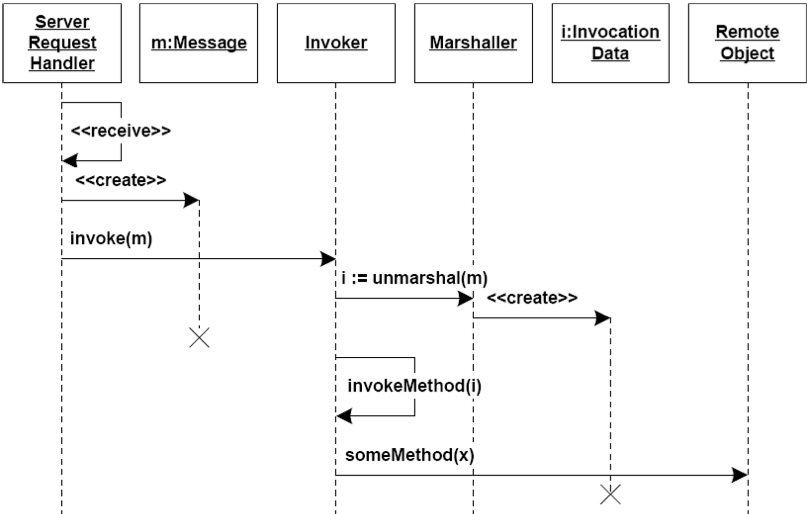
\includegraphics[scale=0.25]{images/invocation-server.png}
\end{center}
\textbf{Remoting Error Propagation:}
\begin{center}
	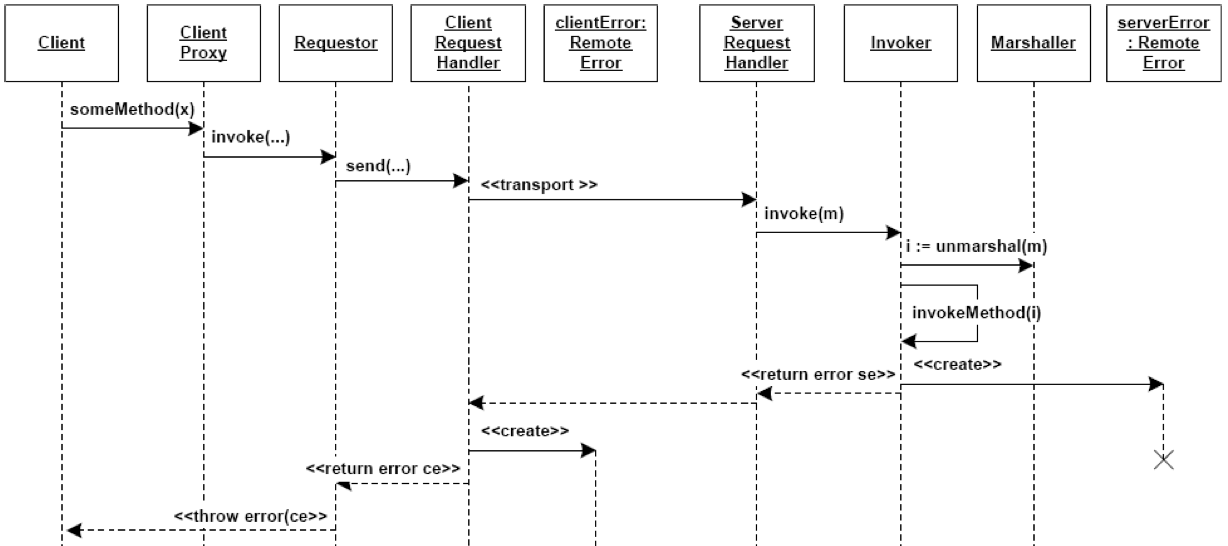
\includegraphics[scale=0.25]{images/remoting-error-propagation.png}
\end{center}
\subsubsection{CLIENT PROXY}
\begin{itemize}
	\item Local object within the client process that offers the same interface as the remote object
	\item Simplifies the usage of the REQUESTOR
	\item Provides type safety on top of the REQUESTOR
	\item CLIENT PROXY is specific to the type of the remote object, typically generated from the INTERFACE DESCRIPTION
	\item Needs to be available on client side, either statically linked or dynamically loaded
\end{itemize}
\begin{center}
	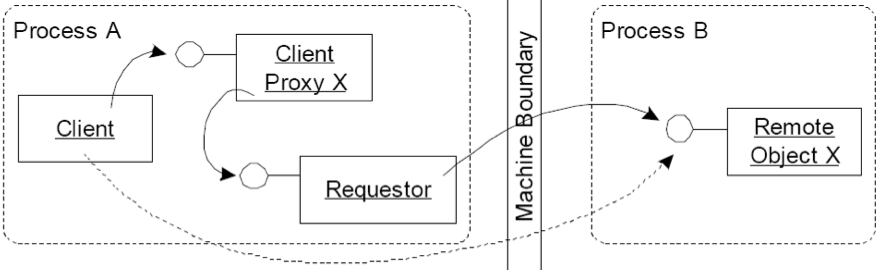
\includegraphics[scale=0.2]{images/client-proxy.png}
\end{center}
\subsubsection{REQUESTOR}
\begin{itemize}
	\item Constructs a remote invocation on the client side from parameters such as remote object location, remote object type, operation name and arguments and sends the invocation to the remote object
	\item Client should not need to perform these tasks itself
\end{itemize}
\begin{center}
	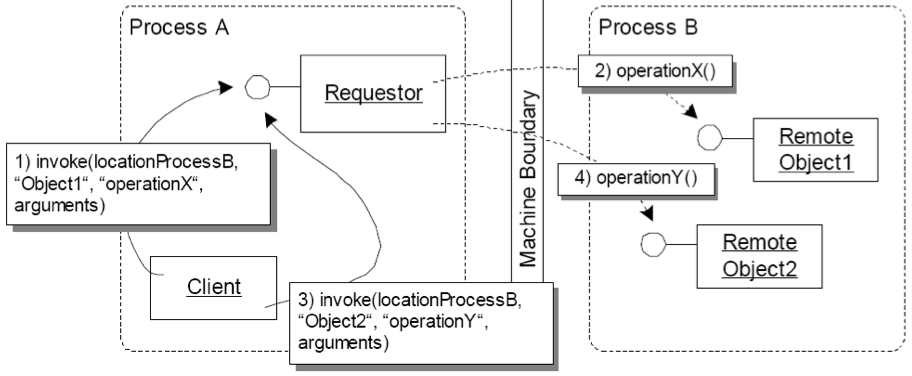
\includegraphics[scale=0.2]{images/requestor.png}
\end{center}
\begin{itemize}
	\item Used by the client directly or by the client proxy object
	\item Tasks
		\begin{enumerate}
			\item Accepts parameters from client (or from client proxy)
			\item Delegates task of marshalling the arguments to the MARSHALLER
			\item Sends the request using the CLIENT REQUEST HANDLER
			\item Throws REMOTING ERRORS in case of communication problems
			\item Delegates task of unmarshalling results to the MARSHALLER
			\item Returns result
		\end{enumerate}
	\item  Independent of the specific remote object details (such as type, etc)
	\item Concurrent access to REQUESTOR needs to be synchronized
\end{itemize}
\subsubsection{CLIENT REQUEST HANDLER}
\begin{itemize}
	\item Responsible for handling network communication in client application
		\begin{itemize}
			\item Opening and closing network connections to server applications
			\item Sending requests and receiving replies
			\item Dispatching replies back to appropriate REQUESTOR (in case of asynchronous invocations)
			\item Handling of timeouts and threading issues
			\item Handling of invocation errors
		\end{itemize}
	\item Connection handling \\
		Connections to a particular server / port may be shared with other invocations
	\item Typically shared between multiple REQUESTORS
	\item Tasks
		\begin{itemize}
			\item Sending of requests
			\item Receiving and dispatching of responses
			\item Handling of timeouts, threading issues, and invocation errors
		\end{itemize}
	\item Deals with all the communication issues of a server application
		\begin{itemize}
			\item Receives messages from the network
			\item Combines the message fragments to complete messages
			\item Dispatches the messages to the correct INVOKER for further processing
		\end{itemize}
\end{itemize}
\begin{center}
	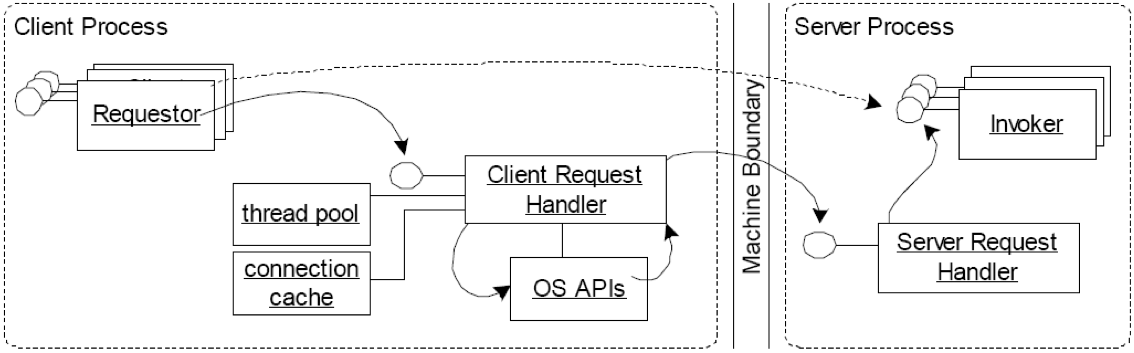
\includegraphics[scale=0.2]{images/client-request-handler.png}
\end{center}
\subsubsection{SERVER REQUEST HANDLER}
\begin{itemize}
	\item Deals with all the communication issues of a server application
		\begin{itemize}
			\item Receives messages from the network
			\item Combines the message fragments to complete messages
			\item Dispatches the messages to the correct INVOKER for further processing
		\end{itemize}
	\item Deals with messages, whereas the INVOKER deals with requests
	\item Must contact the correct INVOKER, i.e. message must contain information about the INVOKER as e.g. a name or ID
	\item Must be able to handle concurrent requests efficiently
		\begin{itemize}
			\item One thread per connection
			\item Connection-independent thread pool
		\end{itemize}
	\item Connection establishment
		\begin{itemize}
			\item New connection for each invocation
			\item Reuse of existing connections (open connections consume resources)		
		\end{itemize}
	\item Tasks
		\begin{enumerate}
			\item Receives data from network and combines them to a complete message
			\item Dispatches the message to the correct INVOKER (uses MARSHALLER to determine the correct INVOKER)
			\item Manages the required resources (connections, threads, ...)
		\end{enumerate}
\end{itemize}
\begin{center}
	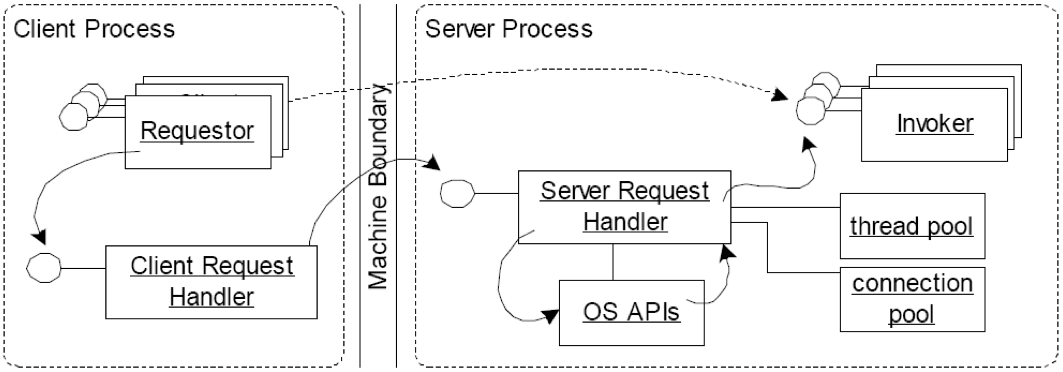
\includegraphics[scale=0.2]{images/server-request-handler.png}
\end{center}
\subsubsection{INVOKER}
\begin{itemize}
	\item Dispatches remote invocations from REQUESTORS to the relevant remote object using the received invocation information
		\begin{itemize}
			\item Static dispatch: generated skeletons
			\item Dynamic dispatch: reflection and dynamic lookup table
		\end{itemize}
	\item Remote object might not be available all the time and only be activated on demand, which requires some part of the system to accept invocations and trigger the (re-)activation of the target remote object
	\item On server side, one or several INVOKER may exist (depends on CONFIGURATION GROUPS)
	\item Low-level network communications are handled by SERVER REQUEST HANDLER
	\item More than one servant might be used to implement a single remote object at runtime ($\Ra$ POOLING) or might have to be activated ($\Ra$ LIFECYCLE MANAGER)
	\item Tasks
		\begin{enumerate}
			\item Accepts parameters from SERVER REQUEST HANDLER
			\item Delegates task of unmarshalling the arguments to the MARSHALLER
			\item Sends the request using the remote object (or its servant)
			\item Delegates task of marshalling results to the MARSHALLER
			\item Returns result to SERVER REQUEST HANDLER
		\end{enumerate}
\end{itemize}
\begin{center}
	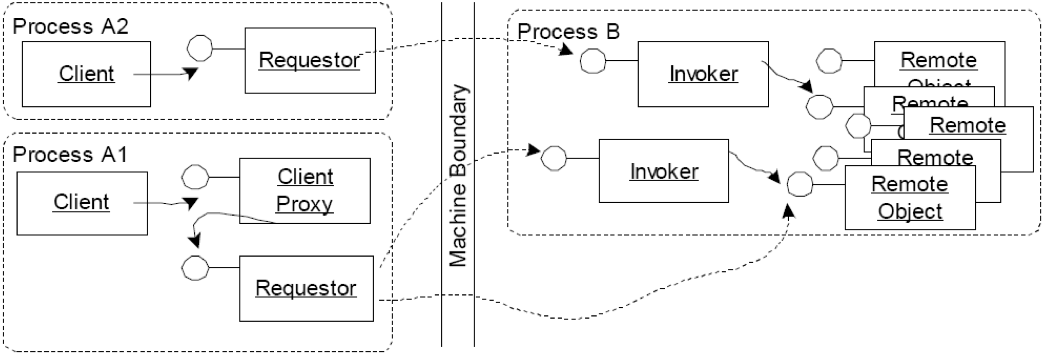
\includegraphics[scale=0.2]{images/invoker.png}
\end{center}
\subsubsection{MARSHALLER}
\begin{itemize}
	\item Used to serialize invocation information into a byte stream (or into XML)
	\item Must be able to handle Cyclic structures, Alias references and Remote references
	\item Conversion from/to byte stream should be defined only once per type
	\item Hooks might be supported to provide custom marshallers
\end{itemize}
\begin{center}
	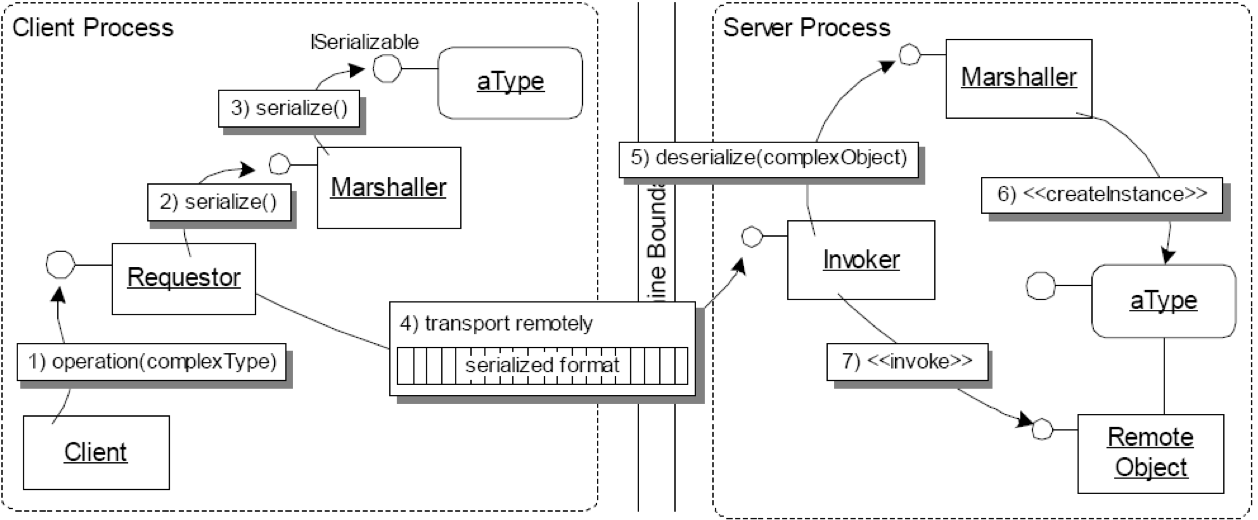
\includegraphics[scale=0.2]{images/marshaller.png}
\end{center}
\subsubsection{INTERFACE DESCRIPTION}
\begin{itemize}
	\item Describes the interface of a remote object
	\item Serves as the contract between CLIENT PROXY and INVOKER.
	\item Client and Server use either code generation or runtime configuration techniques to meet the interface contract
	\item Allows that client and server code are written in different programming languages
\end{itemize}
\begin{center}
	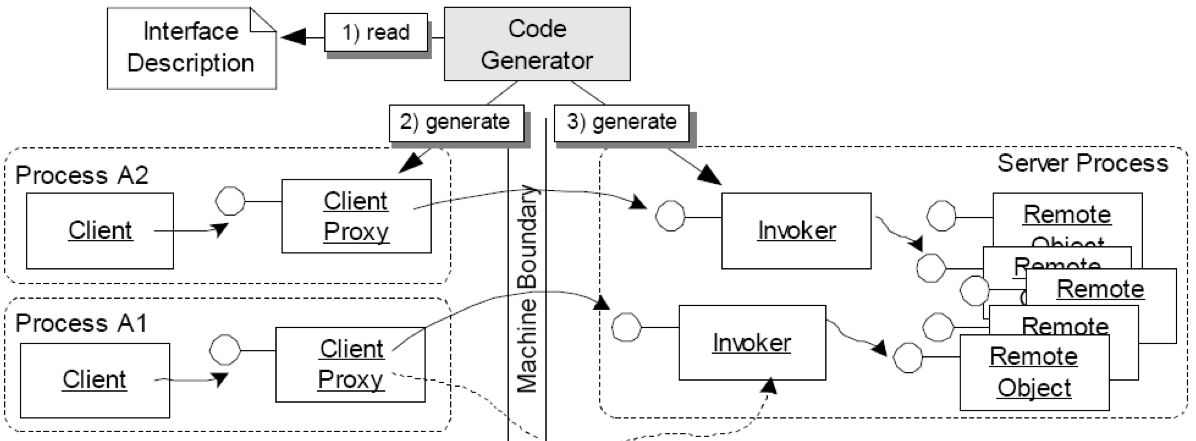
\includegraphics[scale=0.2]{images/interface-description.png}
\end{center}
\subsubsection{REMOTING ERROR}
\begin{itemize}
	\item Used to report problems that occur during a remote invocation, client must be able to distinguish between Distribution/communication related errors and Application-logic related errors
	\item Remoting errors detected inside the server application need to be transported back to the client
	\item Client might handle errors transparently (e.g. invoking another server)
\end{itemize}
\begin{center}
	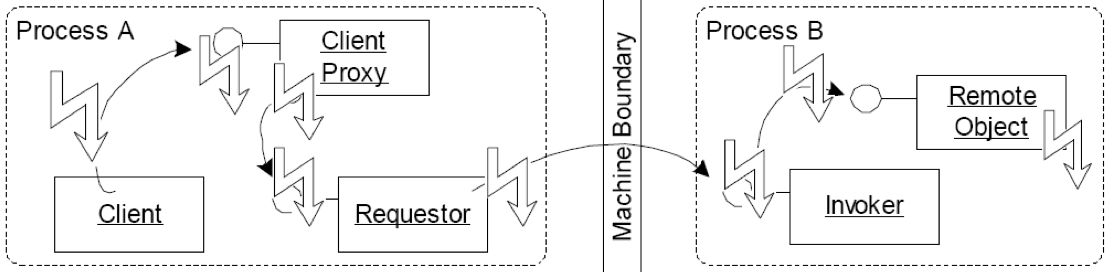
\includegraphics[scale=0.2]{images/remoting-error.png}
\end{center}
\subsection{Identification Patterns}
\subsubsection{Overview}
\begin{center}
	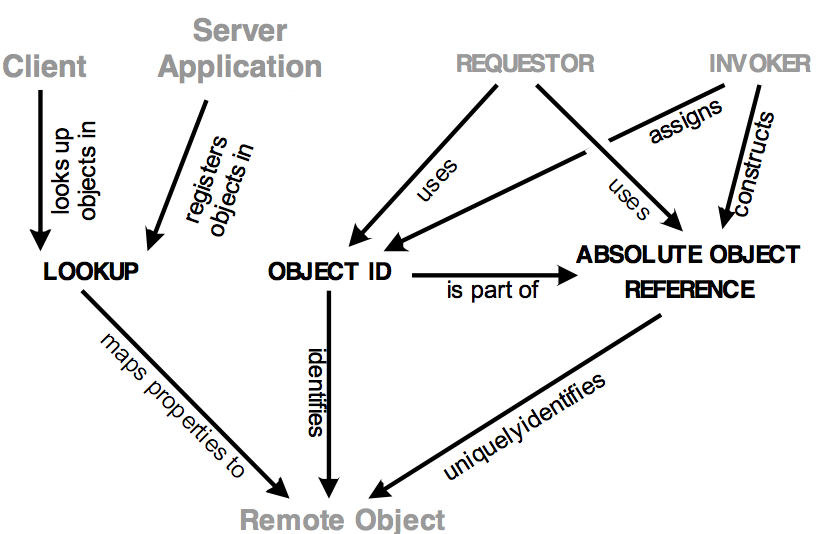
\includegraphics[scale=0.3]{images/identification-patterns.png}
\end{center}
\subsubsection{Interactions}
\textbf{Registration in Lookup:}
\begin{center}
	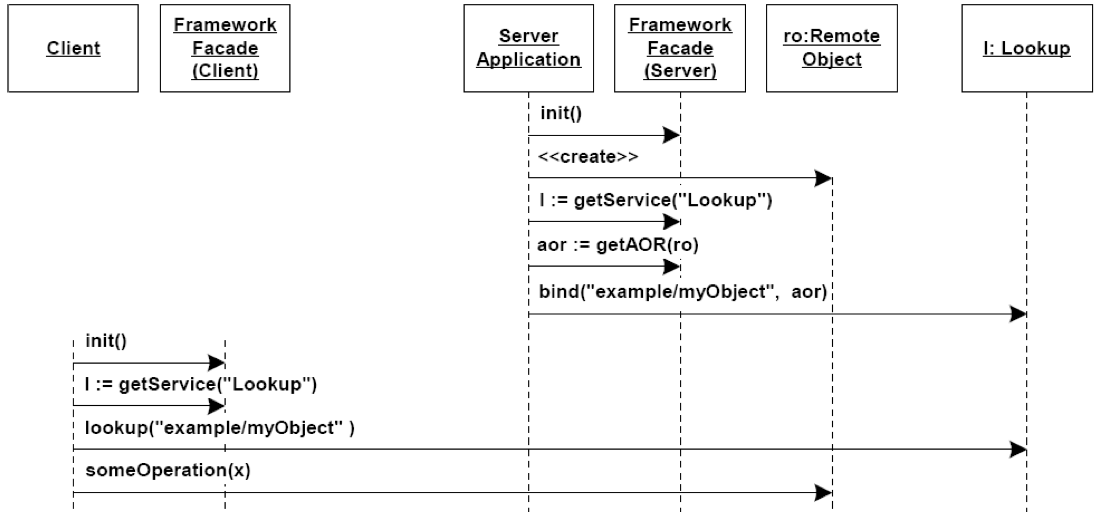
\includegraphics[scale=0.3]{images/interactions-registration.png}
\end{center}
\textbf{Marshalling of absolute object references: p1.anOperation(p2):}
\begin{center}
	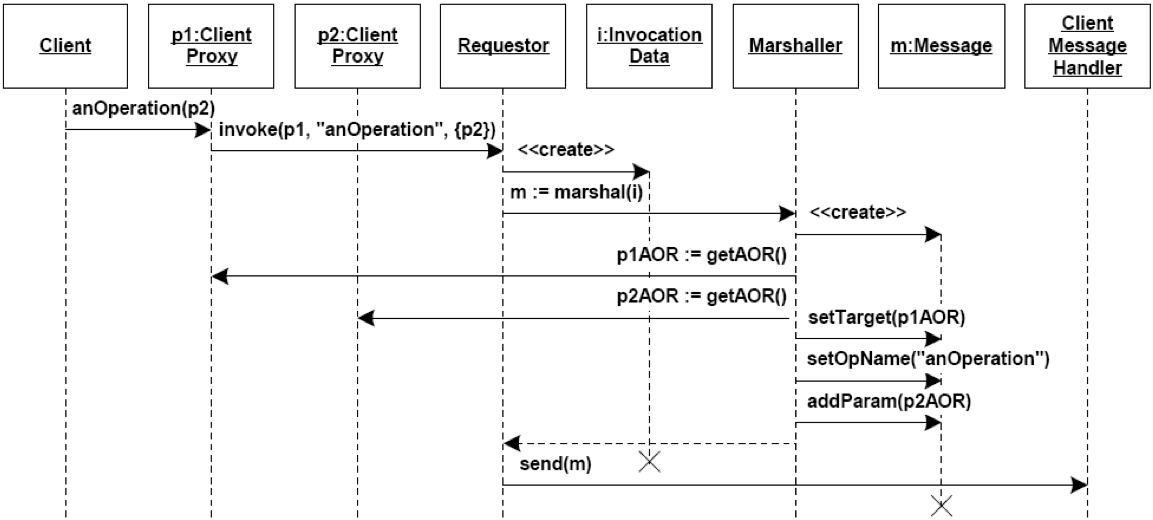
\includegraphics[scale=0.2]{images/interactions-marshalling.png}
\end{center}
\subsubsection{OBJECT ID}
Refer to remote objects, rather than the servants realizing the remote
object at runtime
\begin{center}
	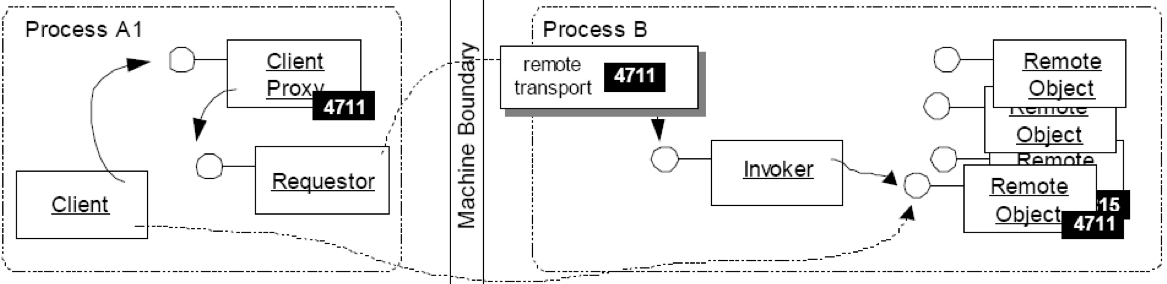
\includegraphics[scale=0.2]{images/objectId.png}
\end{center}
\subsubsection{ABSOLUTE OBJECT REFERENCE}
\begin{itemize}
	\item Contains the information necessary for a client to connect the INVOKER
	\item Uniquely identifies invoker and remote object, typically contains Endpoint information, ID of the INVOKER Object ID
	\item Used by clients to exchange references to remote objects
	\item If several protocols are supported by the server, the protocol to be used by the client has to be included in the reference
	\item May be transient or persistent
		\begin{itemize}
			\item Transient: only valid as long as server has not been restarted
			\item Persistent: valid even after restart of the server application
		\end{itemize}
	\item Client invokes an operation with a reference to another remote object
\end{itemize}
\begin{center}
	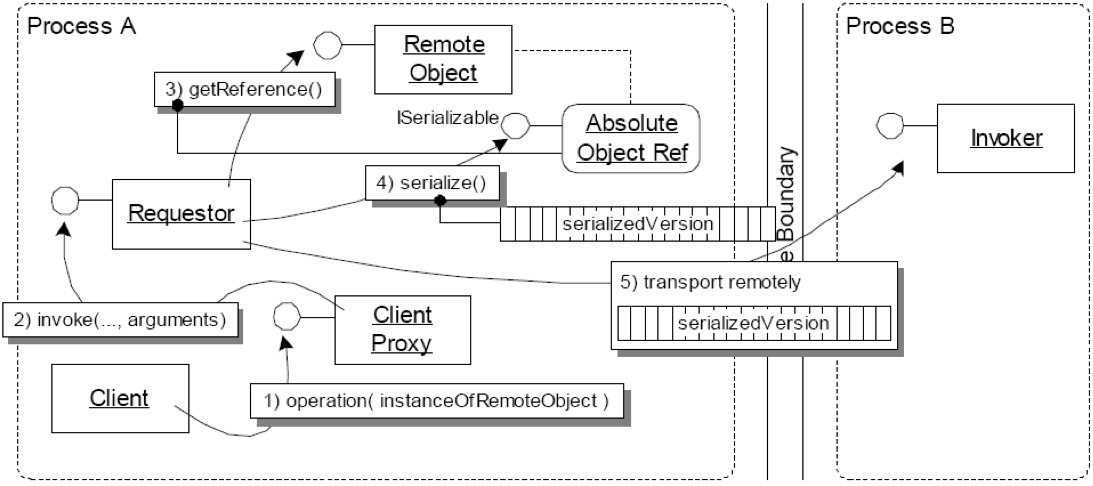
\includegraphics[scale=0.2]{images/absolute-object-reference.png}
\end{center}
\subsubsection{LOOKUP}
\begin{itemize}
	\item Provides ABOLUE OBJECT REFERENCES to remote objects
	\item Associates object references with properties (typically names)
	\item Used by clients to query for object references based on properties
	\item Provides an interface to bind and lookup object references
	\item Implemented as a remote object itself
	\item Only factory objects should be registered in the LOOKUP
\end{itemize}
\begin{center}
	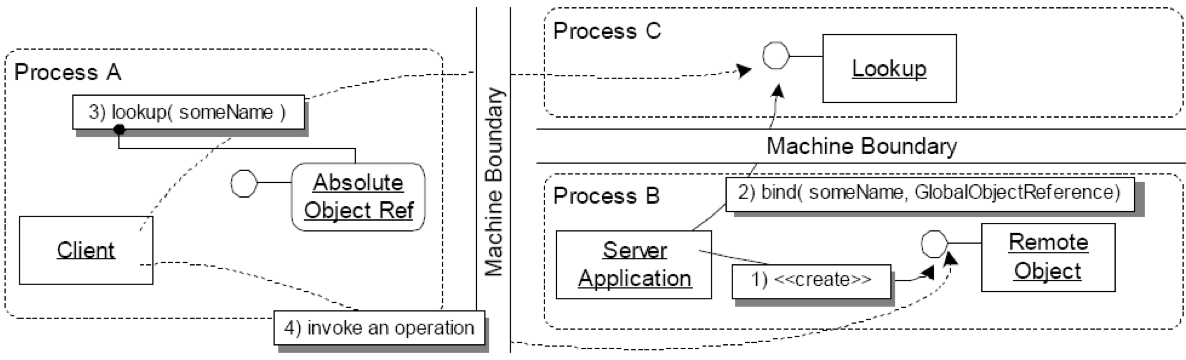
\includegraphics[scale=0.2]{images/lookup.png}
\end{center}
\subsection{Invocation Asynchrony Patterns}
\subsubsection{Overview}
\begin{center}
	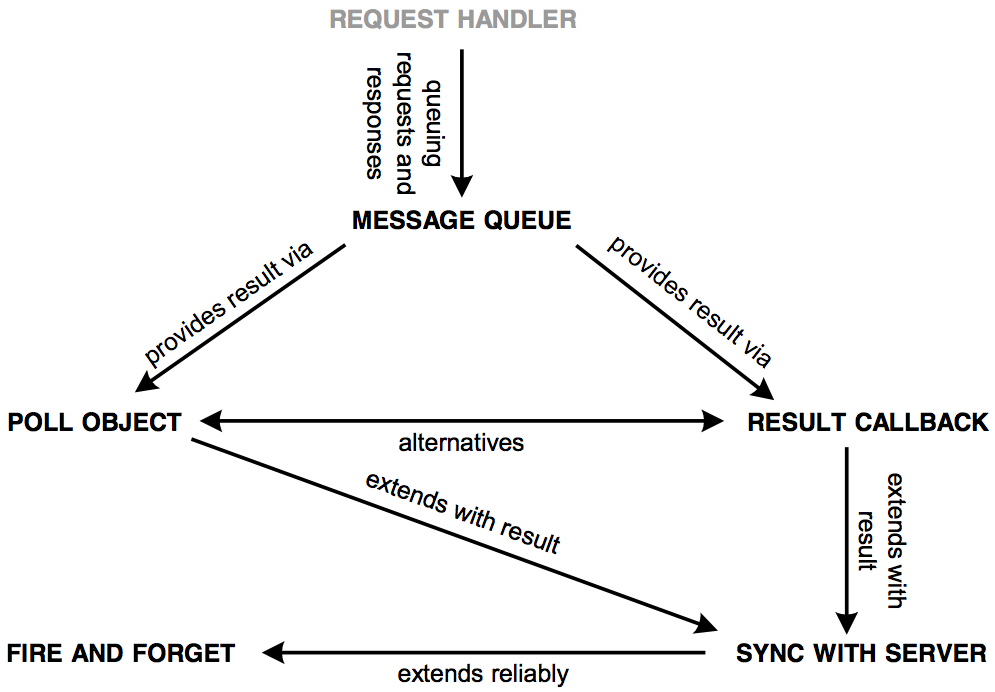
\includegraphics[scale=0.3]{images/invocation-asynchrony-patterns.png}
\end{center}
\subsubsection{FIRE AND FORGET}
\begin{itemize}
	\item Requestor sends the invocation across the network and returns control immediately to the caller
	\item Applicable if
		\begin{itemize}
			\item Client does neither expect a return value (void method) nor an exception
			\item Client simply needs to notify remote object of an event
			\item Reliability of the invocation is not critical (client does not get an acknowledgement from remote object)
		\end{itemize}
\end{itemize}
\begin{center}
	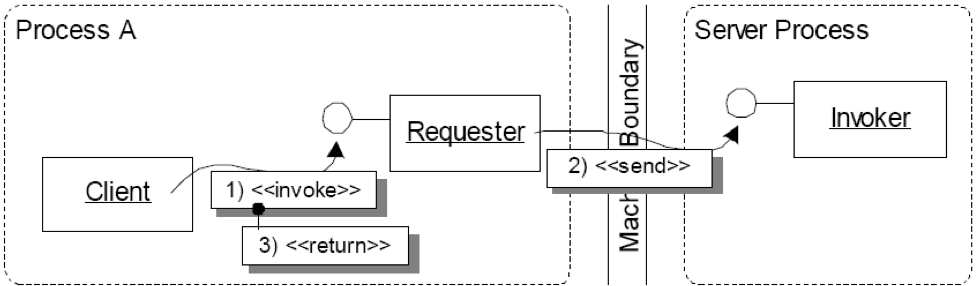
\includegraphics[scale=0.2]{images/fire-and-forget.png}
\end{center}
\subsubsection{SYNC WITH SERVER}
\begin{itemize}
	\item Requestor sends the invocation across the network and waits for a reply from the server acknowledging the successful receipt of the invocation
	\item Acknowledgement is returned before operation is performed on server
	\item Applicable if
		\begin{itemize}
			\item Client does neither expect a return value (void method) nor an exception
			\item Fire-and-forget is too unreliable
		\end{itemize}
\end{itemize}
\begin{center}
	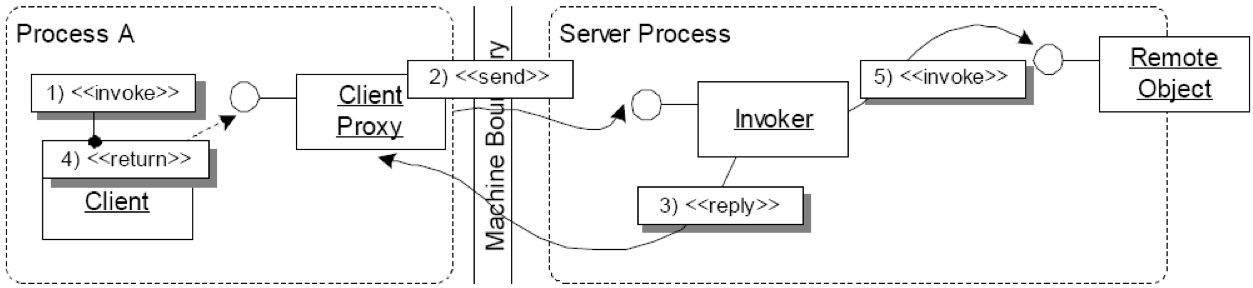
\includegraphics[scale=0.2]{images/sync-with-server.png}
\end{center}
\subsubsection{POLL OBJECT (Future)}
\begin{itemize}
	\item Requestor returns poll object immediately which is used by client to query result (client may block on poll object until result is available)
	\item Client can continue with other tasks asynchronously as long as result is not available on poll object
	\item Applicable if Client does not need result immediately to continue its execution
\end{itemize}
\begin{center}
	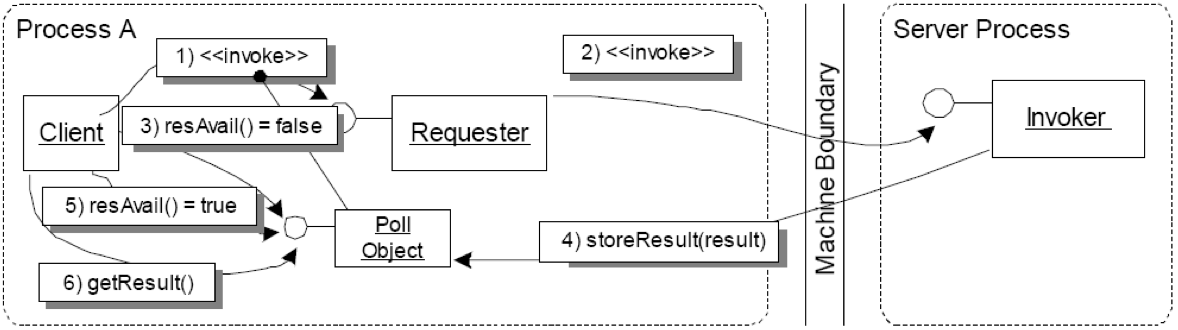
\includegraphics[scale=0.2]{images/poll-object.png}
\end{center}
\subsubsection{RESULT CALLBACK}
\begin{itemize}
	\item Provides a callback-based interface for remote invocations on the client
		\begin{itemize}
			\item Client passes result-callback to the requestor
			\item Invocation returns immediately after sending the invocation
			\item Callback method is invoked on result-callback when the result is available
		\end{itemize}
	\item Client is informed immediately when the result becomes available
\end{itemize}
\begin{center}
	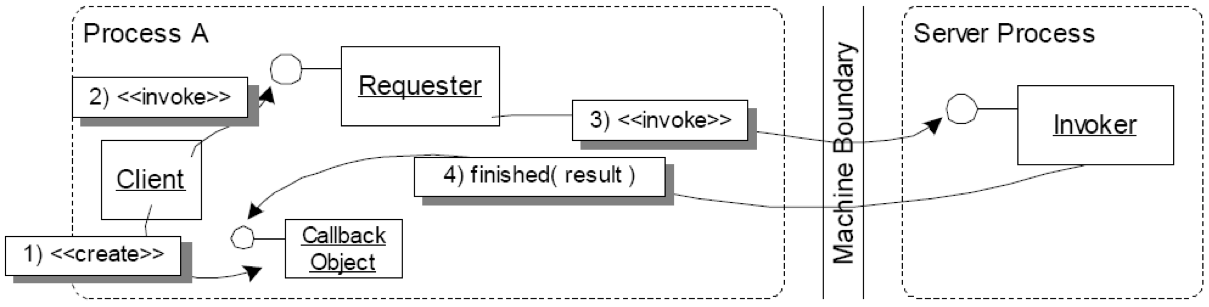
\includegraphics[scale=0.2]{images/result-callback.png}
\end{center}
\subsubsection{MESSAGE QUEUE}
\begin{itemize}
	\item Guarantees invocation and result delivery order
	\item Queues local to client/server request handler (no external message queue)
\end{itemize}
\begin{center}
	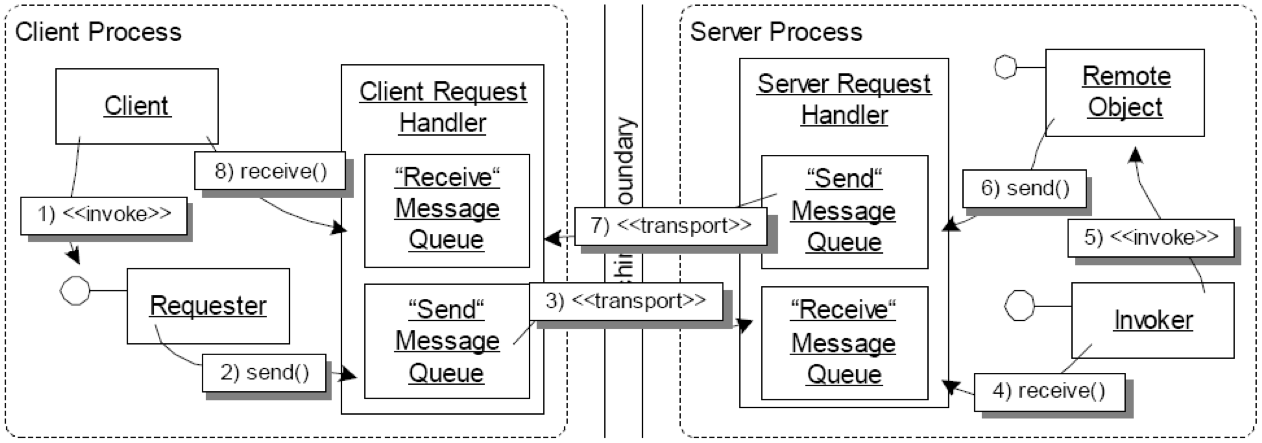
\includegraphics[scale=0.2]{images/message-queue.png}
\end{center}
\subsubsection{Relation among invocation asynchrony patterns}
\begin{center}
	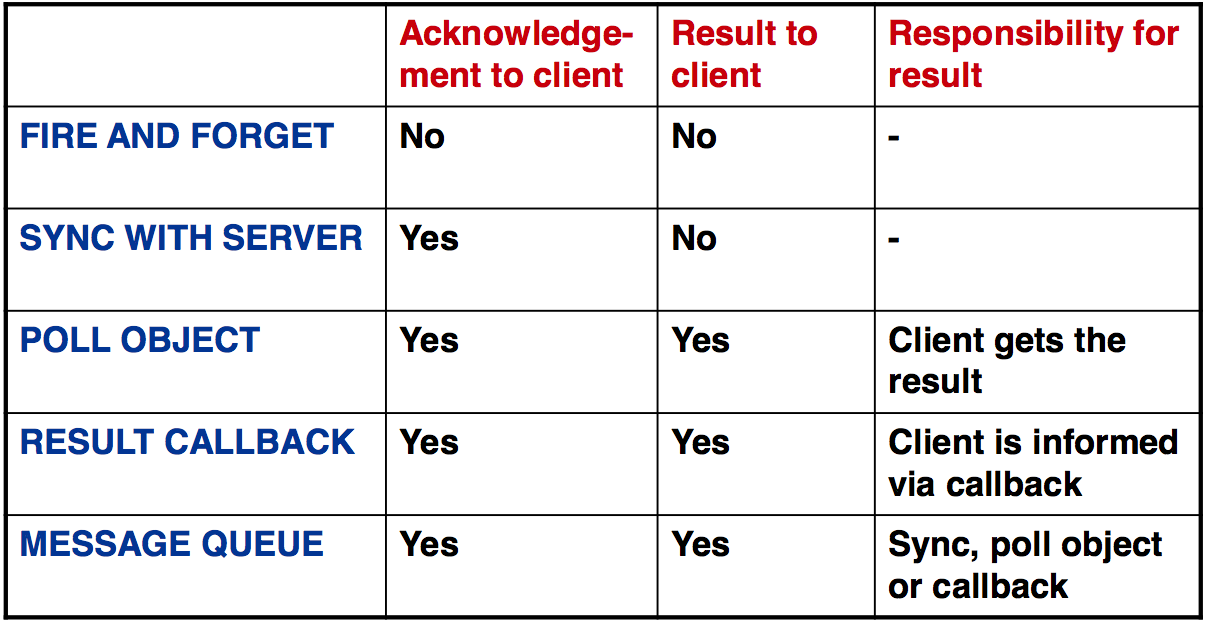
\includegraphics[scale=0.2]{images/asynchrony-pattern-compare.png}
\end{center}
\subsection{Lifecycle Management Patterns}
\begin{center}
	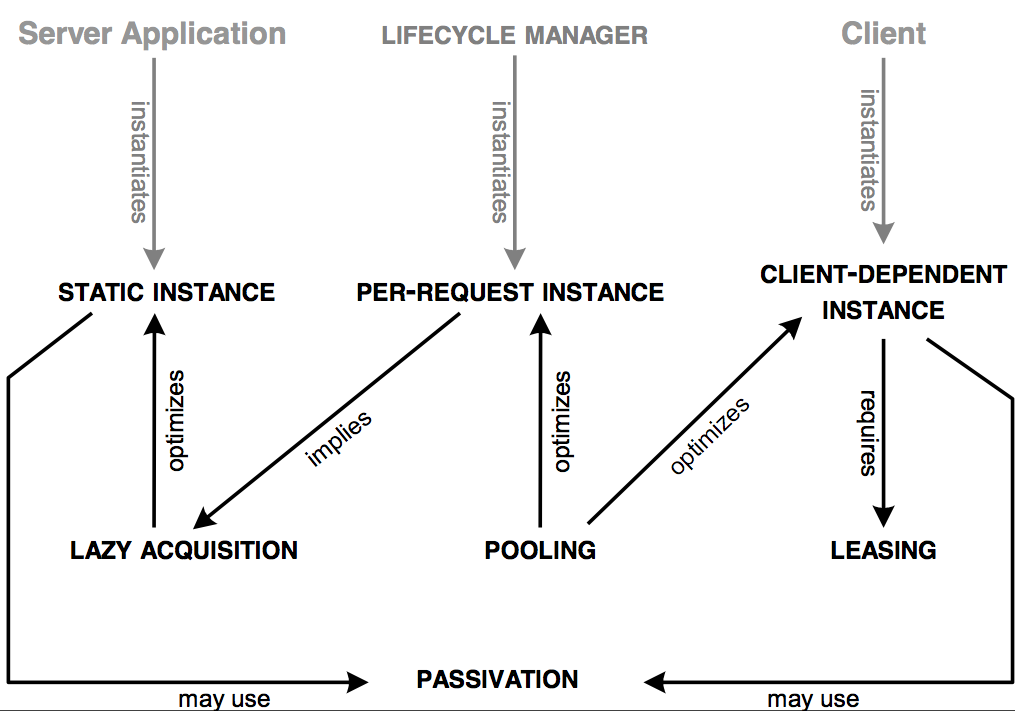
\includegraphics[scale=0.4]{images/lifecycle-management-pattern.png}
\end{center}
\subsection{Extension Patterns}
\begin{center}
	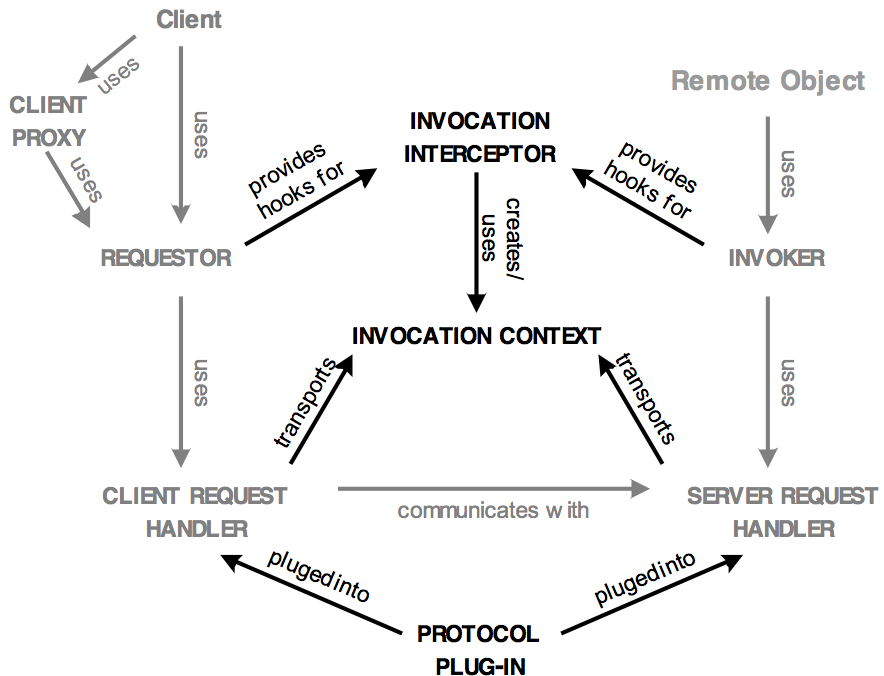
\includegraphics[scale=0.4]{images/extention-pattern.png}
\end{center}

\newpage
\section{Code Samples}
\subsection{Socket}
\lstinputlisting[caption=Client,style=JavaStyle]{code/SocketBankDriver.java}
\lstinputlisting[caption=Server,style=JavaStyle]{code/SocketBankServer.java}
\subsection{Internet}
\lstinputlisting[caption=Client,style=JavaStyle]{code/HttpBankDriver.java}
\lstinputlisting[caption=Server,style=JavaStyle]{code/HttpBankServer.java}
\subsection{XmlRpc}
\lstinputlisting[caption=Client,style=JavaStyle]{code/XmlRpcBankDriver.java}
\lstinputlisting[caption=Server,style=JavaStyle]{code/XmlRpcBankServer.java}
\subsection{REST}
\lstinputlisting[caption=Client,style=JavaStyle]{code/RestBankDriver.java}
\lstinputlisting[caption=Server,style=JavaStyle]{code/RestBankServer.java}
% Inhalt Ende 
\end{document} 